\documentclass[10pt,serif,mathserif,compress,hyperref={colorlinks}]{beamer}
\mode<presentation>
\usepackage{pgf}
\usepackage{pgfpages}
\usepackage[T1]{fontenc}
\usepackage[utf8]{inputenc}

\usepackage{lmodern}
\usepackage{lastpage}
\usepackage{comment}
\usepackage{geometry}
\usepackage[most]{tcolorbox}
\tcbuselibrary{skins}
\usepackage{beamerthemesplit}
\usepackage{amsmath, amsfonts, epsfig, xspace}
\usepackage{pstricks,pst-node}
\usepackage{multimedia}
\usepackage{pifont}   % zapf dingbats
\usepackage{marvosym} % MarVoSym dingbats
\usepackage{wasysym}
\usepackage{animate}

\usepackage{graphicx}% for including figures
\usepackage{tikz}
\usepackage[tikz]{bclogo}
\usetikzlibrary{positioning,decorations.pathreplacing,arrows}
\usepackage{tikzsymbols}
\setlength{\parindent}{0pt}

%%%%%%%%%%%%%%%%%%  Couleurs %%%%%%%%%%%%%%%%%%%%%%%%%%%
\definecolor{mauve}{rgb}{0.5,0,0.7}
\definecolor{carmin}{rgb}{0.7,0,0}
\definecolor{bleu}{rgb}{0,0,0.7}
\definecolor{marron}{rgb}{0.6,0.35,0}
\definecolor{vert}{rgb}{0,0.5,0}
\definecolor{gris}{rgb}{0.9,0.9,0.9}
\definecolor{no}{rgb}{1,0.9,1}
%%%%%%%%%%%%%%%%%%%%%%%%%%%%%%%%%%%%%%%%%%%%%%%%%%%%%%%%%%

\definecolor{White}        {rgb}{1.0,1.0,1.0}

\definecolor{VeryDarkBlue} {RGB}{0,0,153}
\definecolor{DarkBlue}     {rgb}{0.0,0.0,0.6}
\definecolor{Blue}         {rgb}{0.0,0.0,1.0}
\definecolor{MidBlue}      {rgb}{0.6,0.6,1.0}
\definecolor{LightBlue}    {rgb}{0.8,0.8,1.0}
\definecolor{VeryLightBlue}{rgb}{0.9,0.9,1.0}

\definecolor{Gray}{rgb}{0.7,0.7,0.7}
\definecolor{LightGray}{rgb}{0.94,0.94,0.94}

\definecolor{DarkGreen}{rgb}{0,0.6,0}
\definecolor{MidGreen}{rgb}{0.6,1,0.6}
\definecolor{LightGreen}{rgb}{0.88,1,0.88}
\definecolor{VeryLightGreen}{rgb}{0.9,1,0.9}

\definecolor{Yellow}{rgb}{1,1,0.4}
\definecolor{MidYellow}{rgb}{1,1,0.5}
\definecolor{LightYellow}{rgb}{1,1,0.6}
\definecolor{VeryLightYellow}{rgb}{1,1,0.9}

\definecolor{DarkRed}{rgb}{0.7,0.,0.}
\definecolor{Red}{rgb}{0.8,0.,0.}
\definecolor{LightRed}{rgb}{1,0.8,0.8}
\definecolor{VeryLightRed}{rgb}{1,0.9,0.9}

\definecolor{Mauve}{rgb}{0.7,0.,0.7}

\definecolor{Magenta}{rgb}{1,0.,1}
\definecolor{LightMagenta}{rgb}{1,0.5,1}

\definecolor{Chocolate}{rgb}{0.54,0.2,.004}
\definecolor{DarkChocolate}{RGB}{103,38,.00}

\definecolor{DarkOrange}{rgb}{0.65,0.35,0.}
\definecolor{Orange}{rgb}{.9,0.4,0.}
\definecolor{LightOrange}{rgb}{1,0.8,0.5}

%\definecolor{Brown}{rgb}{0.4,0.4,0.}

\definecolor{LightCyan}{rgb}{0.5,1.,1.}

\definecolor{PBG} {rgb}{1.0,1.0,0.6}
\definecolor{PTXT}{rgb}{0.2,0.2,0.0}
\definecolor{IBG} {rgb}{0.8,0.8,1.0}
\definecolor{ITXT}{rgb}{0.2,0.2,0.0}
\definecolor{OBG} {rgb}{0.8,1.0,0.8}
\definecolor{OTXT}{rgb}{0.0,0.4,0.0}

\newcommand{\CommentVeryLightBlue}[1]{{\textcolor{VeryLightBlue}{#1}}}
\newcommand{\CommentWhite}[1]{{\textcolor{White}{#1}}}

\newcommand{\VeryDarkBlue}[1]{\textcolor{DarkBlue}{#1}}
\newcommand{\DarkBlue}[1]{\textcolor{DarkBlue}{#1}}
\newcommand{\Blue}[1]{\textcolor{Blue}{#1}}
\newcommand{\LightBlue}[1]{\textcolor{LightBlue}{#1}}
\newcommand{\VeryLightBlue}[1]{\textcolor{VeryLightBlue}{#1}}

\newcommand{\DarkGreen}[1]{\textcolor{DarkGreen}{#1}}
\newcommand{\LightGreen}[1]{\textcolor{LightGreen}{#1}}
\newcommand{\VeryLightGreen}[1]{\textcolor{VeryLightGreen}{#1}}
\newcommand{\MidGreen}[1]{\textcolor{MidGreen}{#1}}

\newcommand{\DarkRed}[1]{\textcolor{DarkRed}{#1}}
\newcommand{\Red}[1]{\textcolor{red}{#1}}
\newcommand{\LightRed}[1]{\textcolor{LightRed}{#1}}
\newcommand{\VeryLightRed}[1]{\textcolor{VeryLightRed}{#1}}

\newcommand{\Gray}[1]{\textcolor{gray}{#1}}

\newcommand{\Black}[1]{\textcolor{black}{#1}}

\newcommand{\White}[1]{\textcolor{white}{#1}}

\newcommand{\Mauve}[1]{\textcolor{Mauve}{#1}}

\newcommand{\LightMagenta}[1]{\textcolor{LightMagenta}{#1}}
\newcommand{\Magenta}[1]{\textcolor{Magenta}{#1}}

\newcommand{\DarkOrange}[1]{\textcolor{DarkOrange}{#1}}
\newcommand{\Orange}[1]{\textcolor{Orange}{#1}}
\newcommand{\LightOrange}[1]{\textcolor{LightOrange}{#1}}

\newcommand{\DeepPurple}[1]{{\textcolor[rgb]{0.3,0.,0.6}{#1}}}

\newcommand{\Brown}[1]{{\textcolor{Brown}{#1}}}
\newcommand{\Chocolate}[1]{\textcolor{Chocolate}{#1}}
\newcommand{\DarkChocolate}[1]{\textcolor{DarkChocolate}{#1}}

\definecolor{DBluePy}{RGB}{ 28, 78, 99}
\definecolor{BluePy} {RGB}{ 60,110,131}
\definecolor{MBluePy}{RGB}{200,210,240}
\definecolor{LBluePy}{RGB}{220,230,240}
\definecolor{DOranPy}{RGB}{248,194,  3}
\definecolor{OranPy} {RGB}{255,220, 70}
\definecolor{GreenPy}{RGB}{237,255,204}

\newcommand{\bsh}{\textbackslash}
\newcommand{\bshbsh}{\textbackslash\textbackslash}
\newcommand{\chevrons}{\ttfamily>\hspace*{-0.25mm}>\hspace*{-0.25mm}>\hspace*{0.28mm}\xspace}
\newcommand{\M}[1]{\Mauve{#1}}
\newcommand{\DG}[1]{\DarkGreen{#1}}
\newcommand{\DR}[1]{\DarkRed{#1}}
\newcommand{\B}[1]{\Blue{#1}}
\newcommand{\BPy}[1]{\BluePy{#1}}
\newcommand{\VDB}[1]{\VeryDarkBlue{#1}}
\newcommand{\DO}[1]{\DarkOrange{#1}}
\newcommand{\Or}[1]{\Orange{#1}}
\newcommand{\Choco}[1]{\Chocolate{#1}}
\newcommand*{\truc}{\Gray{\textbullet}}

\newcommand{\bif}[1]{{\ttfamily \M{#1}}}	% Python built in function
\newcommand{\typ}[1]{{\ttfamily \M{#1}}}  % Python built in type
\newcommand{\key}[1]{{\ttfamily \Or{#1}}}
\newcommand{\str}[1]{{\ttfamily \DG{#1}}}
\newcommand{\com}[1]{{\ttfamily \DR{#1}}}
\newcommand{\out}[1]{{\ttfamily \B{#1}}}
\newcommand{\command}[1]{{\ttfamily \Choco{#1}}}
\newcommand{\code}[1]{{\ttfamily \Choco{#1}}}
\newcommand{\file}[1]{{\ttfamily \VDB{#1}}}

\newcommand{\bifBF}[1]{\textbf{\bif{#1}}}	% Python built in function
\newcommand{\typBF}[1]{\textbf{\typ{#1}}}  % Python built in type
\newcommand{\keyBF}[1]{\textbf{\key{#1}}}
\newcommand{\strBF}[1]{\textbf{\str{#1}}}
\newcommand{\comBF}[1]{\textbf{\com{#1}}}
\newcommand{\outBF}[1]{\textbf{\out{#1}}}
\newcommand{\commandBF}[1]{\textbf{\command{#1}}}
\newcommand{\codeBF}[1]{\textbf{\code{#1}}}
\newcommand{\fileBF}[1]{\textbf{\file{#1}}}

\newcommand{\bfchoco}[1]{\textbf{\Chocolate{#1}}}
\newcommand{\bfdarkchoco}[1]{\textbf{\DarkChocolate{#1}}}

\usepackage{minted}

\usetheme{jlcKeynote}
\useoutertheme[subsection=false]{miniframes}
\setbeamercolor{background canvas}{bg=gray!50!white}
\setbeamercolor{structure}{bg=white, fg=gray}
\setbeamertemplate{itemize item}{\small\gray{$\CIRCLE$}}
\setbeamertemplate{itemize subitem}{\tiny\gray{$\CIRCLE$}}
\settowidth{\leftmargini}{\usebeamertemplate{itemize item}}
\addtolength{\leftmargini}{\labelsep}

\setbeamercovered{transparent}

\hypersetup{linkcolor=Yellow}
\hypersetup{citecolor=DeepPink4}
\hypersetup{urlcolor=DarkBlue}
\hypersetup{anchorcolor=Magenta}

%=============================== 1 ================================================

\title[\hspace*{.75\linewidth}\insertframenumber/\inserttotalframenumber]
      {\fontsize{18}{18}\selectfont{\textbf{A gentle introduction to\\[2mm]
            Artificial Intelligence \&\\[2mm]
            Machine Learning}}\\[5mm]
      \fontsize{13}{13}\selectfont{DuMAS department day -- 2023/09/22}
}

\subtitle{}

\author[{\tiny{JLC -- Sept23 -- v1.0 }}
  
\hspace*{.75\linewidth}]
%{
\includegraphics[height=2.5cm]{images/logo-am-couleur-72dpi_alpha.jpg}\\[5mm]
{\fontsize{9}{9}\selectfont{\hspace*{-5mm}Jean-Luc.Charles@mailo.com}}

\institute{}

\date{}

\titlegraphic{\vspace*{-1.6cm}
\includegraphics[height=3.cm]{images/robot.png}\\
  \href{https://creativecommons.org/licenses/by-sa/4.0/}
       {
\includegraphics[height=5mm]{images/CC-BY-SA.jpeg}}     
}

\logo{}

\tcbset{enhanced, boxrule=0.2pt, sharp corners, drop lifted shadow,
    width=1.0\textwidth, left=5pt, left skip=-20pt,
    colback=Chocolate!25!white,colframe=Chocolate!75!black}

\renewcommand\ttdefault{lmtt}

\begin{comment}
v1.2 -- JLC :
>>> Modification des tcolorbox pour les avoir :
- plus larges (width=...)
- mieux centrées dans la page  (left skip=...)
- avec moins de marge à gauche (left=...)
\end{comment}

\begin{document}

\frame[plain]{\titlepage}

\newcommand{\boldtt}[1]{{\ttfamily\bfseries #1}}

\setbeamercolor{structure}{fg=gray!50!white}

\section{Welcome}

%=============================== 2 ================================================
\begin{frame}{An introduction to AI \& Machine Learning}
  
  %\vspace*{-3mm}%
  \begin {bclogo}[noborder=true, couleur=gray!50, couleurBarre=Chocolate, logo=\bctrombone, marge=0, margeG=-0.5]
    {\ Some points of interest}
    \medskip
    \begin{itemize}
    \item Preliminaries: the historical way...
    \item \Chocolate{Unsupervised} / \Chocolate{Supervised} / \Chocolate{Reinforcement} learning
    \item Use a \Chocolate{Virtual Python Environment} (PVE) to work on ML
    \item {[}{\it If needed}...{]} more technical slides are available in the appendix for those who want to know more
    \end{itemize}
  \end{bclogo}
  
  \visible<2->{
    \begin {bclogo}[noborder=true, couleur=gray!50, couleurBarre=Chocolate, logo=\bctrombone, margeG=-0.5]
      {\ My profile}
    \medskip
      \begin{itemize}
      \item I'm teaching Python programming (Scientific \& Object Oriented)
      \item I started to get interested in ML in 2015
      \item I wrote several materials in ML : workshop, project \& practical work
        for different shools (ENSAM, ENSEIRB, ENSPIMA, PPU...)
      \end{itemize}
    \end{bclogo}
  }

\end{frame}
%===============================================================================

\section{Some preliminaries}

\subsection{The historical way}

%================================ 3 ============================================
\begin{frame}{The historical way...}
  \hspace*{-2mm}from: \href{https://medium.com/analytics-vidhya/brief-history-of-neural-networks-44c2bf72eec}
    {Kate Strachni: "Brief History of Neural Netowrks", medium.com}\\[1mm]
  \hspace*{-8mm}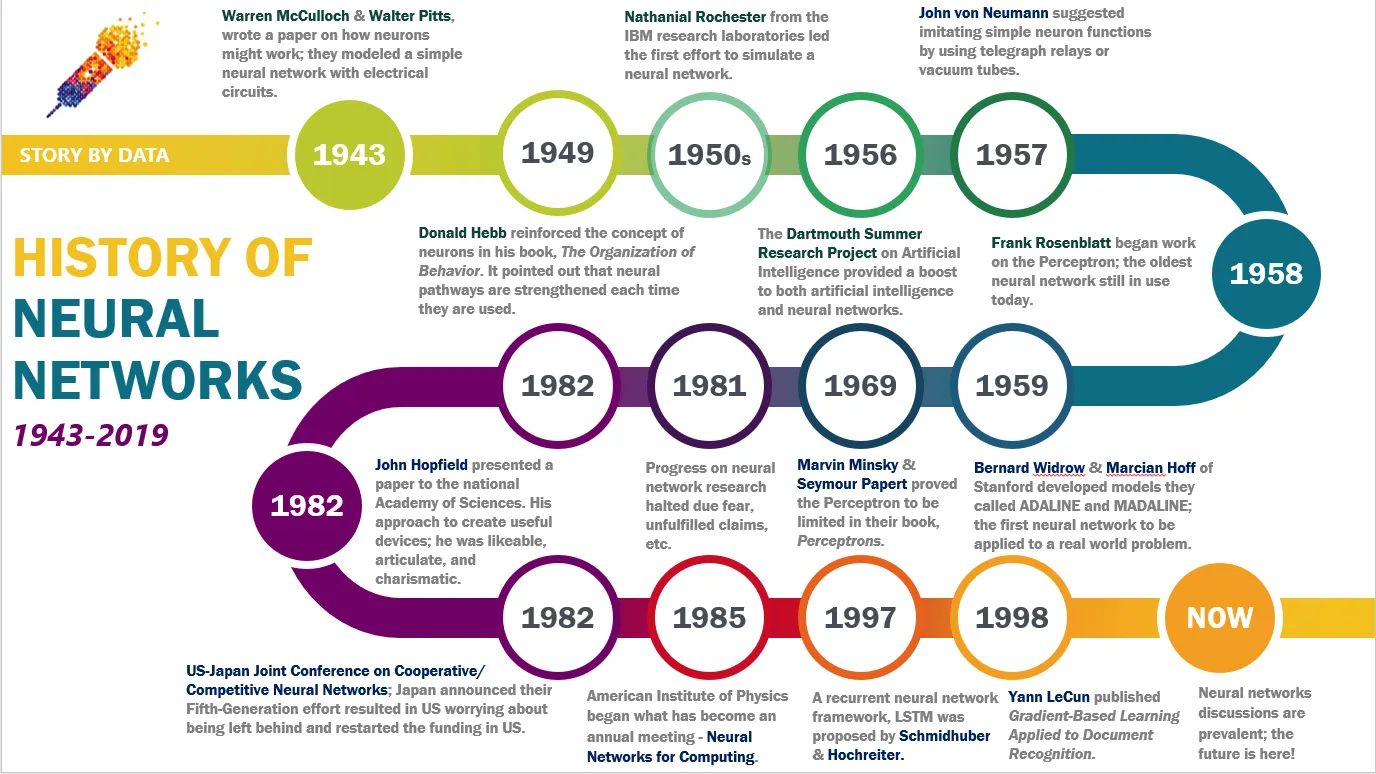
\includegraphics[width=1.15\textwidth]{images/Brief History of NN - Kate Strachnyi.png}
\end{frame}
%===============================================================================

%================================ 4 ============================================
\begin{frame}{The historical way...}
  \hspace*{-2mm}from: \href{https://pub.towardsai.net/a-brief-history-of-neural-nets-472107bc2c9c}
    {Pumalin: "A Brief History of Neural Nets", medium.com}\\[1mm]
  \hspace*{-8mm}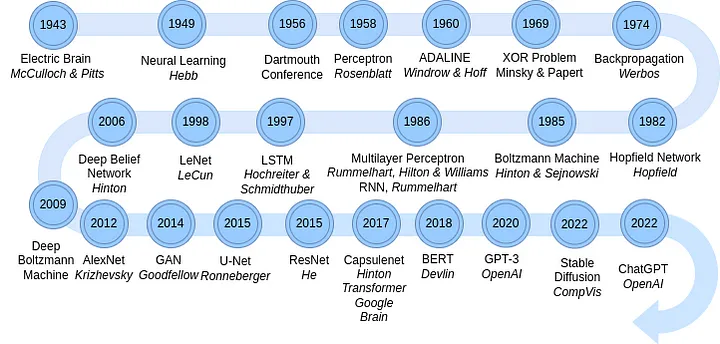
\includegraphics[width=1.15\textwidth]{images/A brief History of NN - Pumalin.png}
\end{frame}
%===============================================================================

%================================ 5 ============================================
\begin{frame}{The historical way...}
  \hspace*{-2mm}from: \href{https://towardsdatascience.com/ten-years-of-ai-in-review-85decdb2a540}
    {Thomas A Dorfe: "Ten Years of AI in Review", medium.com}\\[1mm]
  \hspace*{-6mm}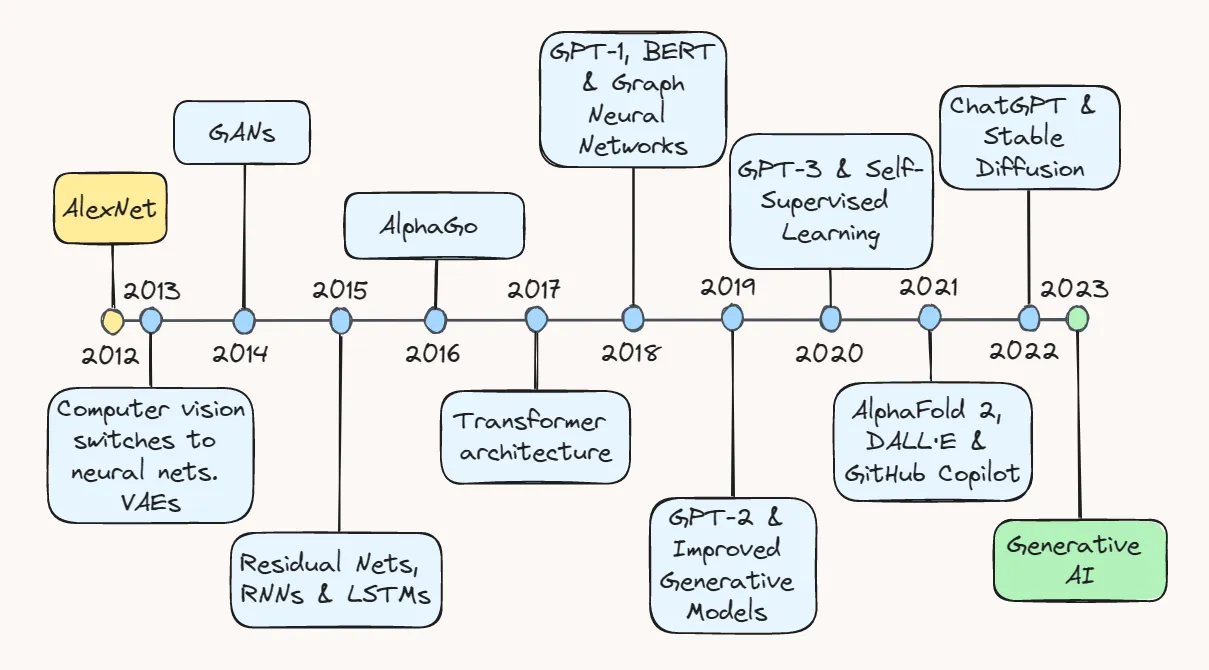
\includegraphics[width=1.1\textwidth]{images/Ten Years of AI in Review.png}
\end{frame}
%===============================================================================

%================================ 6 ============================================
\begin{frame}{Artificial Intelligence ?}

  \vspace*{-1mm}
  \begin {bclogo}[noborder=true, couleur=gray!50, couleurBarre=Chocolate, logo=\bctrombone, margeG=-0.5]
    {}
    \vspace*{-5mm}
    Historically\footnote{{\tiny first used in 1956 by \href{https://en.wikipedia.org/wiki/John\_McCarthy\_\%28computer\_scientist\%29}{John McCarthy},
    researcher at Stanford during the Dartmouth conference}} {\it badly chosen} term!\\
    Ambiguous current meaning...\\
    Many (contradictory) definitions depending on periods and authors...
    \end{bclogo}
  \medskip
  \begin{itemize}
    {\small
    \item {\em ''...the science of making computers do things that require intelligence when done by humans.}''
      {\tiny \href{http://www.alanturing.net/turing\_archive/pages/reference\%20articles/what\%20is\%20ai.html}{Alan Turing, 1940}}
      
    \item {\em ''the field of study that gives computers the ability to learn without being explicitly programmed.''}
      {\tiny  \href{http://infolab.stanford.edu/pub/voy/museum/samuel.html}{Arthur Samuel, 1960}}
      
    \item {\em ''A computer program is said to learn from experience E with respect to some class of tasks T and performance measure P,
      if its performance at tasks in T, as measured by P, improves with experience E.''}
      {\tiny \href{https://www.cs.cmu.edu/~tom/}{Tom Mitchell, 1997}}
      
    \item Notion of {\em intelligent agent} or {\em rational agent}\\
      {\em ''...agent that acts in such a way as to
        reach the best solution or, in an uncertain environment, the best predictable solution.}''\\
      {\tiny  \hyperlink{refRusselNorvig}{Stuart Russel, Peter Norvig, ``Intelligence Artificielle'' 2015}}
    }
  \end{itemize}
  
\end{frame}
%===============================================================================

%================================= 7 ===========================================
\begin{frame}{Artificial Intelligences ?}
 
  \textbf{Strong AI}

  \visible<1->{%
    \begin{itemize}
    \item Build systems that think exactly the same way that people do.
    \item Try also to explain how humans think... \Chocolate{Whe are not yet here}.
    \end{itemize}
  }

  \textbf{Weak AI}
  
  \visible<1->{% 
    \begin{itemize}
    \item Build systems that can behave like humans.
    \item The results will tell us nothing about how humans think.
    \item \Chocolate{We already are there}... We use it every day!\\
      (anti-spam, facial/voice recognition, language translation...)
    \end{itemize}
  }

  \textbf{General AI}
  \visible<1->{%
    \begin{itemize}
    \item AI systems designed for the ability to reason in general.
    \end{itemize}
  }

  \textbf{Narrow AI}
  \visible<1->{%
    \begin{itemize}
    \item AI systems designed for specific tasks.
    \end{itemize}
  }
  
\end{frame}
%===============================================================================

\section{ML}

\subsection{ML Branches}

%================================== 8 ==========================================
\begin{frame}{Branches of Machine Learning}

  {\small Page from \href{https://medium.com/machine-learning-for-humans/why-machine-learning-matters-6164faf1df12}
  {medium.com/machine-learning-for-humans/...}}\\[2mm]
  
  \hspace*{-10mm}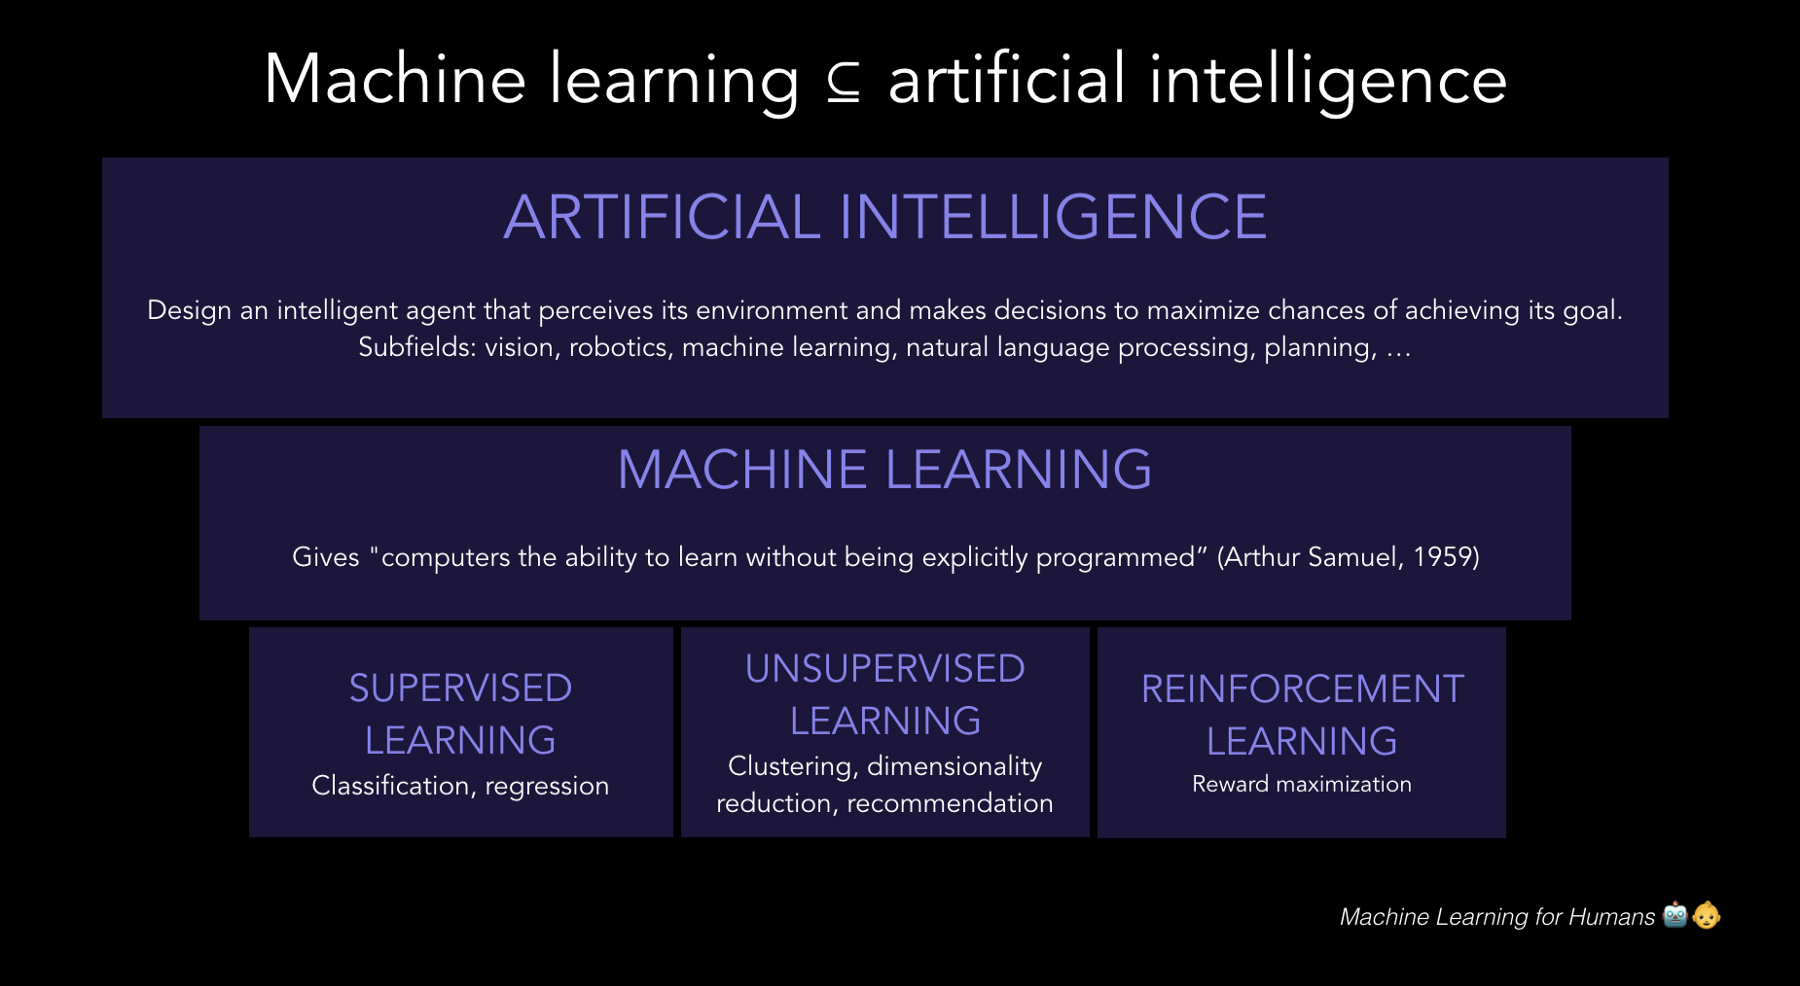
\includegraphics[width=1.2\textwidth]{images/AI-from_MachineLearningForHumans.png}
  \vspace*{-8mm}
  
\end{frame}
%===============================================================================

%================================== 9 ==========================================
\begin{frame}{Branches of Machine Learning}

  %% Excellent: https://www.ibm.com/cloud/learn/machine-learning?lnk=fle

  \begin{tcolorbox}[title={\bf Supervised learning}]
    {\bf labeled dataset} is used to train algorithms:
    \begin{itemize}
    \item \textbf{Classification}
      \begin{itemize}
      \item Images classification
      \item Objects detection in images
      \item Speech recognition...
      \end{itemize}
    \item \textbf{Regression}
      \begin{itemize}
      \item Predict a value...
      \end{itemize}
    \item \textbf{Anomaly detection}
      %% anomaliy detection with supervised laerning suppose that there are no "new annomaly" in the
      %% datat set to process, because the anomalies have been learned and the algorithm will not
      %% recognize new anomaly that was not learned...
      \begin{itemize}
      \item Spam detection
      \item Manufacturing: finding known (learned) defects
      \item Weather prediction
      \item Diseases classification...
      \end{itemize}        
    \end{itemize}
    \vspace*{-1mm}$\cdots$
  \end{tcolorbox}
  
\end{frame}
%===============================================================================

%=================================== 10 ========================================
\begin{frame}{Branches of Machine Learning}
  \begin{tcolorbox}[title={\bf Unsupervised learning}]
    Analyze and cluster \textbf{unlabeled datasets}:
    \begin{itemize}
    \item \textbf{Clustering} \& \textbf{Grouping} 
      \begin{itemize}
      \item Data mining, web data grouping, news grouping...
      \item Market segmentation
      \item Astronomical data analysis...
      \end{itemize}        
    \item \textbf{Anomaly Detection}
      \begin{itemize}
      \item Fraud detecion
      \item Manufacturing: finding defects even new ones
      \item Monitoring abnormal activity: failure, hacker, fraud...
      \item Fake account on Internet...
      \end{itemize}
    \item \textbf{Dimensionality reduction}
      \begin{itemize}
      \item Compress data using fewer numbers...
      \end{itemize}
    \end{itemize}
    \vspace*{-1mm}$\cdots$
  \end{tcolorbox}    
\end{frame}
%===============================================================================

%=================================== 11 ========================================
\begin{frame}{Branches of Machine Learning}  
  \begin{tcolorbox}[title={\bf Deep Reinforcement Learning} DRL]
    An agent (the Neural Network) learns how to drive an environment by maximising a \textbf{reward}:
    \begin{itemize}

    \item \textbf{Control/command}
      \begin{itemize}
      \item Controlling \href{run:./videos/trained-PPO-example.webm}{robots}, drones, \href{run:./videos/DRL-Cartpole.webm}{mecatronic systems}
      \item Factory optimization
      \item Financial (stock) trading...
      \end{itemize}        
    \item \textbf{Decision making}
      \begin{itemize}
      \item games (video games)
      \item financial analysis...
      \end{itemize}
    \end{itemize}
    \vspace*{-1mm}$\cdots$
  \end{tcolorbox}    
\end{frame}
%===============================================================================

\subsection{ML algorithms}

%=================================== 12 ========================================
\begin{frame}{}

  %See \href{https://www.ibm.com/cloud/learn/machine-learning}{www.ibm.com/cloud/learn/machine-learning}
  
  \begin{tcolorbox}[title=Various approaches for ML algorithms]
    {\small
      \begin{minipage}[t]{.55\textwidth}
        \bfdarkchoco{Supervised learning:}
        \begin{itemize}
        \item<1-> \only<1>{\Blue{Neural Networks}}\only<2>{\Blue{\bf Neural Networks}}
        \item<1> Bayesian inference
        \item<1> Random forest
        \item<1> Decision Tree
        \item<1> Support Vector Machine (SVM)
        \item<1> K-Nearest Neighbor
        \item<1> Linear regression
        \item<1> Logistic regression
        \item<1>...
        \end{itemize}
      \end{minipage}\begin{minipage}[t]{.55\textwidth}
        \bfdarkchoco{Unsupervised learning:}
        \begin{itemize}
        \item<1-> \only<1>{\Blue{Neural Networks}}\only<2>{\Blue{\bf Neural Networks}}
        \item<1> Principal Composant Analysis
        \item<1> Singular Value Decomposition
        \item<1> K-mean \& Prob. clustering
        \item<1>...
        \end{itemize}
        \medskip
        \bfdarkchoco{Reinforcement learning:}
        \begin{itemize}
        \item<1-> \only<1>{\Blue{Neural Networks}}\only<2>{\Blue{\bf Neural Networks}}(Q-learning, Actor-Critic, DDPG, PPO...)
        \item<1> Monte Carlo
        \item<1> SARSA
        \item<1>...
        \end{itemize}
        
      \end{minipage}
    }
  \end{tcolorbox}    
  \visible<2->{This introduction deals only with \Blue{\bf Artificial Neural Networks}.}
\end{frame}
%===============================================================================

\subsection{Fields of ML}

%=================================== 13 ========================================
\begin{frame}{Fields \& applications of ML}

  \begin{tcolorbox}[height=6cm, add to width=.7cm, title=Computer Vision]
    \begin{minipage}[t][][t]{.6\textwidth}
      \begin{itemize}
      \item<1-> Image Classification
      \item<2-> Object Detection 
      \item<3-> (Semantic) Segmentation
      \item<4-> Image Generation\\
        {\small \href{https://www.leptidigital.fr/productivite/meilleurs-generateurs-images-ia-30857/}{Les 10 Meilleurs Générateurs d’Images}}
      \item<5-> Pose Estimation
      \item<5-> ...
      \end{itemize}
    \end{minipage}\begin{minipage}[t][][b]{.4\textwidth}
      \only<1>{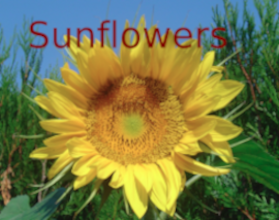
\includegraphics[width=1.\textwidth]{images/image_classification_sunflowers.png}}
      \only<2>{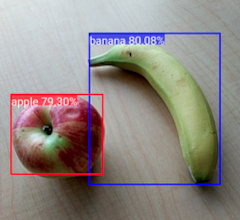
\includegraphics[width=1.\textwidth]{images/object_detection_aple-banana.png}\\[-2mm]
        {\centerline{\tiny Image credit: \href{https://www.tensorflow.org/lite/examples/object_detection/overview}{Tensorflow}}}}
      \only<3>{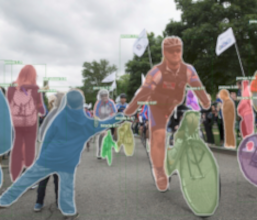
\includegraphics[width=1.\textwidth]{images/image_segmentation_Detectron.png}}
      \only<4>{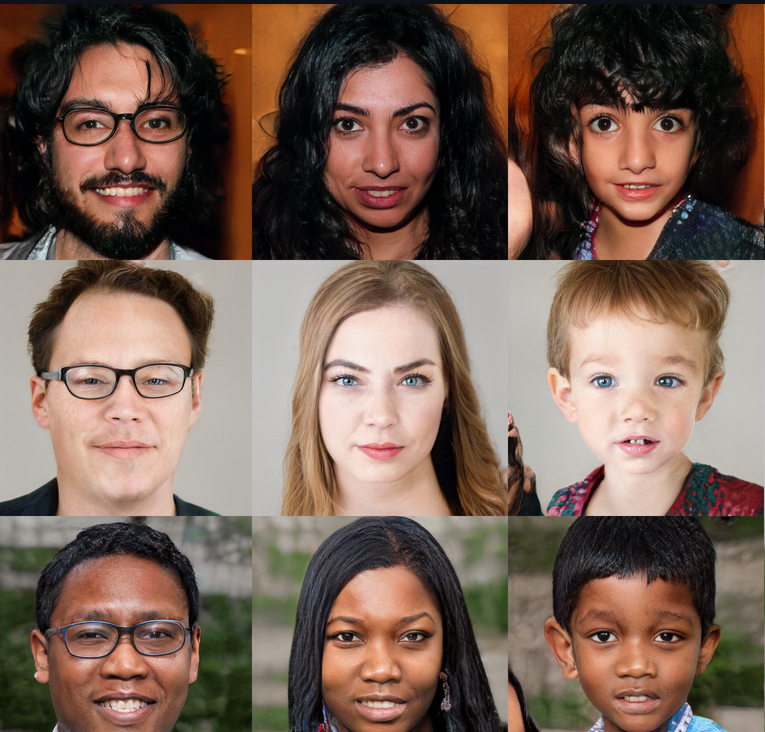
\includegraphics[width=1.\textwidth]{images/image_generation.png}\\[-2mm]
        {\centerline{\tiny Image credit: \href{https://github.com/NVlabs/stylegan}{stylegan}}}}
      \only<5>{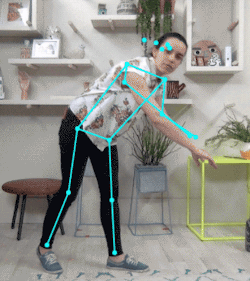
\includegraphics[width=1.\textwidth]{images/pose_estimation_TF.png}\\[-2mm]
        {\centerline{\tiny Image credit: \href{https://www.tensorflow.org/lite/examples/pose_estimation/overview}{Tensorflow-Pose Estimation}}}}
    \end{minipage}
  \end{tcolorbox}
  
\end{frame}
%===============================================================================

%=================================== 14 ========================================
\begin{frame}{Fields \& applications of ML}

  \begin{tcolorbox}[title=Natural Language Processing: NLP]
    \begin{itemize}
    \item<1-> Natural Language Understanding (NLU) 
    \item<1-> Natural Language Generation (NLG)
    \item<1-> Speech recognition / Speech Synthesis (Text To Speech)
    \item<1-> Machine Translation (languages)
    \item<1-> Virtual agents and ChatBots
    \item<1-> Optical character recognition (OCR)
    \item<1-> ...
    \end{itemize}
  \end{tcolorbox}   
  
\end{frame}
%===============================================================================

\subsection{Neural Networks achitectures}

%Physics-Informed Machine Learning Models

%=================================== 15 ==========================================
\begin{frame}{Neural Network Architectures}

Common NN architectures:
\begin{itemize}
  \item \bfdarkchoco{Feed Forward}: the simplest NN made of successive layers of neurones, with {\em Feed Forward} and {\em Back Propagation} algorithms.
  \item \bfdarkchoco{Convolutional} (CNN): Mostly used for analyzing and classifying images.
  \item \bfdarkchoco{Recurrent} (RNN): Used to learn from time series, like the Long Short-Term Memory (LSTM) algorithm.
  \item \bfdarkchoco{Transformers} : Recently used for Natural Language Processing and then for image classification.
  \item \bfdarkchoco{Auto Encoder} (AEN): Dimensionality reduction, Feature extraction, Denoising of data/images, Imputing missing data.
  \item \bfdarkchoco{Generative Adversarial} (GAN): to generate text, images, music...
  \item \bfdarkchoco{Large Language Model} (LLM): read texte, sound, write books, images, speak, make music ...ChatGPT
\end{itemize}
{\small\centering[Synthetic Graphical chart: \href{https://chart-studio.plotly.com/~SolClover/90.embed?autosize=true&referrer=https\%3A\%2F\%2Ftowardsdatascience.com\%2F}{from Saul Dobilas on Medium}] }
\end{frame}
%===============================================================================

\section{PVE}

\subsection{Motivation}

%=================================== 16 ========================================
\begin{frame}{The need of PVE (Python Virtual Environment) to develop ML programs with Python}

  \visible<2->{
  \begin{tcolorbox}[title=Advantages]
    \begin{itemize}
    \item <2-> Dedicated environment (disk tree) with fixed version of the Python interpreter and modules
    \item <3-> Easy to create and destroy if needed
    \item <4-> Each Python project can have its own PVE \\
      \visible<5->{
        $\leadsto$ \DarkGreen{you can load/update modules for a project without breaking other projects}
        }
    \item <6->  PVEs protect your projects against operating system updates or hazardous manipulations...
    \end{itemize}
  \end{tcolorbox}
  }
  \visible<7->{
    \bigskip
  \begin{tcolorbox}[title=Disadvantages]
    \begin{itemize}
    \item <7-> ? (just do it)
    \end{itemize}
  \end{tcolorbox}
  }

\end{frame}
%===============================================================================

%=================================== 17 ========================================
\begin{frame}{PVE: simple to create \& use}
  
  \begin{tcolorbox}[add to width=.7cm, title=Create/populate a PVE with {\bf conda}]
    \begin{itemize}
    \item <1-> Download \& install \href{https://docs.conda.io/en/latest/miniconda.html}{miniconda} for your OS.
    \item <2-> \code{\$ conda create -n dumas1 python=3.8} $\leadsto$ {\small creates the \DarkRed{\boldtt{dumas1}} PVE}
    \item <3-> \code{\$ conda activate dumas1} $\leadsto$ {\small activates the \DarkRed{\boldtt{dumas1}} PVE }
    \item <4-> \code{\$ conda env update -n dumas1 --file <file.yml>} $\leadsto$ {\small loads all the Python modules listed in \file{file.yml} into the \DarkRed{\boldtt{dumas1}} PVE }
    \item <5-> If needed: \code{\$ conda install <module>} or \code{\$ pip install <module>} {\small $\leadsto$ adds a module to the {\bf activated} \DarkRed{\boldtt{dumas}} PVE.}
    \end{itemize}
  \end{tcolorbox}    

  {\small
  \visible<6->{
  \begin{tcolorbox}[add to width=.7cm, title=Advantages / disadvantages]
    \visible<6->{\dSmiley[1.][green!60!white] The version of Python in a conda PVE can be $\neq$ version of the interpreter that comes with the OS installation\\[1mm]}
    \visible<7->{\dSmiley[1.][green!60!white] Some modules installed with \Chocolate{conda} can be more performant\\(numpy \& tensorflow are linked with the \href{https://www.intel.com/content/www/us/en/developer/tools/oneapi/onemkl.html}{MKL} library)\\}
    \visible<8->{\dSadey[1.][red!60!white] \Chocolate{conda install} and \Chocolate{pip install} can be conflicting...}
  \end{tcolorbox}
  }
  }
\end{frame}
%===============================================================================

%=================================== 18 ========================================
\begin{frame}{PVE: simple to create \& use}
  
  \begin{tcolorbox}[add to width=.7cm, title=Create/populate a PVE with {\bf venv}]
    
    \begin{itemize}
    \item <1-> \code{\$ pip install venv} $\leadsto$ {\small Installs the \href{https://docs.python.org/3/library/venv.html}{venv} Python module}
    \item <2-> \code{\$ python -m venv dumas1} $\leadsto$ {\small creates the PVE named \DarkRed{\boldtt{dumas1}}}
    \item <3-> \code{\$ source ./dumas1/bin/activate} $\leadsto$ {\small activates the \DarkRed{\boldtt{dumas1}} PVE }
    \item <4-> \code{\$ pip install -r <requirements.txt>} $\leadsto$ {\small loads all the Python modules listed in \file{requiremnts.txt} into the \DarkRed{\boldtt{dumas1}} PVE }
    \item <5-> \code{(dumas1) \$ pip install <module>}\\
      $\leadsto$ {\small installs a module for the {\bf activated} \DarkRed{\boldtt{dumas1}} PVE}\\
      $\leadsto$ {\small note the path prefix \code{(dumas1)} showing the activated PVE}
    \end{itemize}
    
  \end{tcolorbox}    

  {\small
  \visible<6->{
  \begin{tcolorbox}[title=advantages / disadvantages]
    \visible<6->{\dSadey[1.][red!60!white] The version of Python for the PVE is the version of the interpreter that comes with the OS installation\\[1mm]}
    \visible<7->{\dSmiley[1.][green!60!white] No conflict with \Chocolate{conda install}}
  \end{tcolorbox}
  }}
\end{frame}
%===============================================================================

%===============================================================================
\begin{frame}[fragile]
\frametitle{Installation of Python modules}

\hspace*{-5mm}Examples of files to install some Python modules in the \DarkRed{\boldtt{dumas1}} PVE:\\[-5mm]
  \hspace*{5mm}\begin{minipage}[t]{.35\linewidth}
    \begin {bclogo}[noborder=true, couleur=gray!50, couleurBarre=Chocolate, logo=\bctrombone, marge=0, margeG=-.8]
    {\small YAML format for \codeBF{conda}}
    \begin{minted}[frame=single, fontsize=\footnotesize]{yaml}
name: dumas1
channels:
  - defaults
dependencies:
  - python=3.8
  - tensorflow==2.8.*
  - pandas
  - matplotlib
  - opencv
  - jupyter
  - notebook
  - scikit-learn
  - seaborn
  - pip
\end{minted}
    \end{bclogo}
  \end{minipage}
\hspace*{25mm}\begin{minipage}[t]{.3\linewidth}
    \begin {bclogo}[noborder=true, couleur=gray!50, couleurBarre=Chocolate, logo=\bctrombone, marge=0, margeG=-.8]
    {\small TXT format for \codeBF{pip}}
\begin{minted}[frame=single, fontsize=\footnotesize]{text}
tensorflow==2.8.*
pandas
matplotlib
opencv
jupyter
notebook
scikit-learn
seaborn
\end{minted}
    \end{bclogo}
    \end{minipage}  

\end{frame}
%===============================================================================

%=================================== 18 ========================================
\begin{frame}{PVE: simple to create \& use}
  
  \begin{tcolorbox}[title=the winning recipe]
    
    \begin{itemize}
    \item <1-> \Chocolate{Python Virtual Environment} for every ML project
    \item <2-> \Chocolate{Git} repository (GitHub, GitLab...) for storing, sharing \& versionning the project files
    \item <3-> \Chocolate{requirement.txt} to install the Python modules in the required version for each project
    \item <4-> \Chocolate{Jupyter notebook} and/or \Chocolate{Visual studio code} ({\it aka} VSCode) to developp Python programs.
    \item <5-> Like many IDEs \Chocolate{VSCode} is aware of PVEs.
      
    \end{itemize}
    \end{tcolorbox} 
\end{frame}
%===============================================================================

\section{Reproducibility of training}

\subsection{Motivation}

%=================================== nn ========================================
\begin{frame}{Reproducibility of training}
  
  \begin{tcolorbox}[title=Where to find randomness in NN training]
    
    \begin{itemize}
    \item<1-> \bfdarkchoco{Random initialization of the weights} of the network before the training starts.
    \item<2-> Regularization, e.g. {\bf dropout}, which involves randomly dropping nodes in the network while training.
    \item<3-> Optimization process like {\bf stochastic gradient descent} or {\bf Adam} also include randomness.
    \item<4-> Shuffling of data to build batches to train the NN
    \item<5-> and many others stages in ML algorithms  where random genertaors are used...
    \end{itemize}
  \end{tcolorbox}
    
\end{frame}
%===============================================================================
 
\subsection{Practical work with tensorflow}

%=================================== nn ========================================
\begin{frame}{Reproducibility of training}
  
  \begin{tcolorbox}[title=Practical work with tensorflow]
    
    \begin{itemize}
    \item<1-> We will run a \bfdarkchoco{Jupyter notebook} to illustrate the {\it Reproducibility of training} with {\bf tensorflow}.
    \item<2-> See the PVE usage
    \item<3-> Create a simple {\it Feed Forward} dense network and train it to classify {\it hand written} images form the MNIST
    \item<4-> Explore where and how the question of the Reproducibility occurs... and how to solve it \dSmiley[1.][green!60!white]
    \end{itemize}
  \end{tcolorbox}

    
\end{frame}
%===============================================================================
 
\subsection{References}

%===============================================================================
\begin{frame}{}
  
  \noindent\fontsize{8}{8}\selectfont{

    \hspace*{-4mm}\hypertarget{refRusselNorvig}{[1] }%
    {\em Artificial Intelligence: A Modern Approach (4th Edition)}, By Stuart Russell \& Peter Norvig. 
    Pearson, 2020. ISBN 978-0134610993. \href{http://aima.cs.berkeley.edu/}{aima.cs.berkeley.edu}\\[3mm]
    {\em Intelligence artificielle -- Une approche moderne -- 4e éd.}, By Stuart Russell \& Peter Norvig. 
    Translated by L. Miclet, F. Popineau, \& C. Cadet. Paris: Pearson Education France, 2021. ISBN 978-2326002210.\\[5mm]


    \hspace*{-4mm}\hypertarget{refStrongWeak-AI}{[2] }%
    {\em What is artificial intelligence (AI), and what is the difference between general AI and narrow AI?}, Kris Hammond, 2015\\
    \href{https://www.computerworld.com/article/2906336/what-is-artificial-intelligence.html}
         {www.computerworld.com/article/2906336/what-is-artificial-intelligence.html}\\[5mm]

    \hspace*{-4mm}\hypertarget{StanfordEncyc}{[3] }%
    {\em Stanford Encyclopedia of Philosophy},
    \href{https://plato.stanford.edu/entries/artificial-intelligence}
         {plato.stanford.edu/entries/artificial-intelligence}\\[5mm]

    \hspace*{-4mm}\hypertarget{DeepLeraning}{[4] }%
    {\em  Deep Learning.}, Goodfellow, Ian; Bengio, Yoshua; Courville, Aaron (2016), MIT Pres, ISBN 9780262035613
  }
  
\end{frame}
%===============================================================================

\section{Appendices}

\subsection{The artificial neuron}

%===============================================================================
\begin{frame}{Artificial Neural Networks}
  
  \tikzset{%
  neuron/.style={
    circle,
    draw,
    minimum size=1cm,
    font=\large
  },
  squa/.style={
    draw,
    inner sep=2pt,
    font=\large,
    join = by -latex
  },
  }
  \begin{tcolorbox}[title=The Artificial neuron model]  
    \hspace*{-.7cm}
    \begin{tikzpicture}[x=1.4cm, y=1.cm]

      \node [label=above:\parbox{2cm}{\centering Input\\stimuli}] at (0, 1.5) (x1)  {$x_1$};
      \node [] at (0, 0.5) (x2) {$x_2$};
      \node [] at (0, -0) (vdots) {$\vdots$};
      \node [] at (0, -0.7) (xn) {$x_n$};
      \node [label=above:\parbox{2cm}{\centering Bias}] at (2, 2) (bias) {$b$};
      \node [label=above:\parbox{2cm}{\centering Output}] at (4, 0.15) (y) {$y = f(\sum_i{w_{i}\,x_i} - b)$};
      
      \node [neuron/.try] (output) at (2,0.15) {\large{$\displaystyle{\Sigma | f}$}};
      
      \draw [o-latex] (x1) -- (output);
      \draw [o-latex] (x2) -- (output);
      \draw [o-latex] (xn) -- (output);
      \draw [o-latex] (bias) -- (output);
      \draw [->] (output) -- (y);

      \node [] at (1,1) () {$w_1$} ;
      \node [] at (1,.5) () {$w_2$} ;
      \node [] at (1, -0.45) () {$w_n$} ;
    \end{tikzpicture}
  \end{tcolorbox}
  \smallskip
  \visible<1->{An \bfdarkchoco{artificial neuron}:
    \begin{itemize}
    \item <1-> receives the input stimuli $(x_{i})_{i=1..n}$ with \textbf{weights} $(w_i)$
    \item <1-> computes the \textbf{weighted sum} of the input $\sum_i{w_{i}\,x_i - b}$
    \item <1-> outputs its activation $f(\sum_i{w_{i}\,x_i} - b)$, computed with a non-linear \textbf{activation function} $f$ .
    \end{itemize}
  }

\end{frame}
%===============================================================================

\subsection{Activation functions}

%===============================================================================
\begin{frame}{Artificial Neural Networks}
  
  \begin{tcolorbox}[title={Common activation functions}]
    \hspace*{-5mm}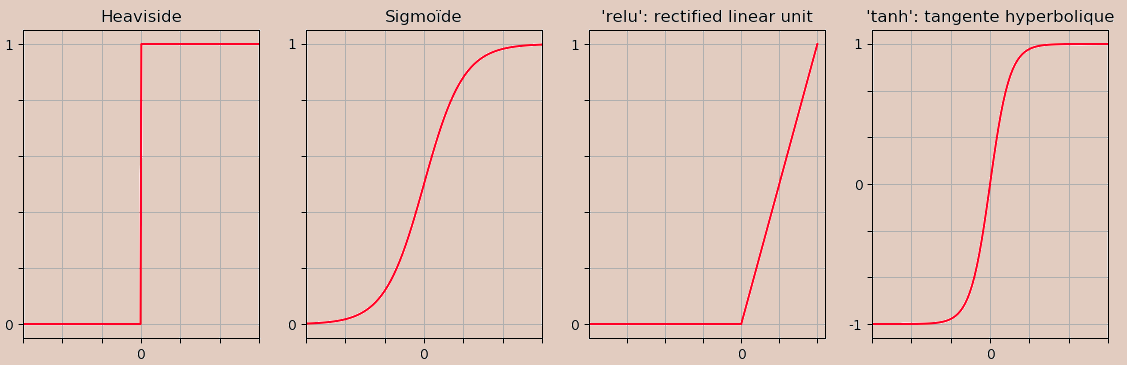
\includegraphics[width=1.1\textwidth]{images/activ_functions-2.png}
  \end{tcolorbox}
  
  \begin{itemize}
  \item Introduces a non-linear behavior.
  \item Sets the range of the neuron output: $[-1, 1]$, $[0, 1]$, $[0, \infty[$...
    \item The bias $b$ sets the activation threshold of the neuron.
  \end{itemize}
  
\end{frame}
%===============================================================================

\subsection{Activation functions SoftMax}

%===============================================================================
\begin{frame}{Réseau de neurones dense}
  \vspace*{-2mm}

  \begin{itemize}
    
  \item Dans les couches intermédiaires la fonction d'activation \bfdarkchoco{relu} favorise l'apprentissage du réseau
    \footnote{{\tiny évite le {\em vanishing gradient} qui apparaît dans
        l'algorithme de {\em back propagation}}}.

  \item La classification (dernière couche) utilise la fonction \bfdarkchoco{softmax} :

  \end{itemize}

    
  \begin{tcolorbox}[title=Fonction d'activation {\em softmax}]  

    \begin{minipage}{.45\textwidth}
      \hspace*{-5mm}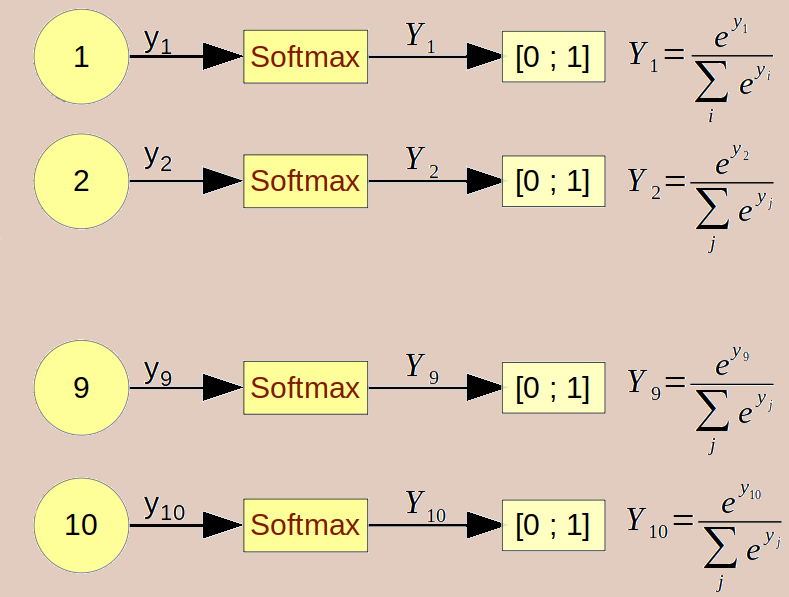
\includegraphics[width=1.\textwidth]{images/softmax-2.png}
    \end{minipage}
    \begin{minipage}{.6\textwidth}
      {\small
        \begin{itemize}
        \item L'activation du neurone $k$ est $Y_k = e^{y_k}/\sum_i{e^{y_i}}$ 
          avec $y_k = \sum_i \omega_i x_i - b$ calculé par le neurone $k$.
        \item Les sorties des neurones s'interprètent comme des probabilités dans l'intervalle [0,1].
        \end{itemize}
      }
    \end{minipage}
  \end{tcolorbox}

  \vspace*{-1mm}
  \visible<2>{Réponse du réseau $\leadsto$ label associé au neurone de plus grande probabilité.}

\end{frame}
%===============================================================================

\subsection{One-hot coding}

%===============================================================================
\begin{frame}{Réseau de neurones dense}

  \begin{tcolorbox}[title=Codage {\em One-hot} des labels]  

    Mettre les labels des images au format de la sortie du réseau :

    {\small
        \begin{itemize}
        \item Labels des images  : \textbf{nombres entiers} de 0 à 9.
        \item Sortie du réseau : \textbf{vecteur de 10 \texttt{float}} dans l'intervalle [0,1] calculés par les fonctions {\em softmax} des 10 neurones de sortie.
        \item Codage {\em one-hot} d'un ensemble ordonné $\mathfrak{L}$ de $N$ labels : \\[1mm]
          - chaque label est représenté par un vecteur à $N$ composantes toutes nulles, sauf une (égale à $1$),\\
          - le rang du $1$ du vecteur associé à un label est le rang du label dans $\mathfrak{L}$.
        \end{itemize}
      }
  \end{tcolorbox}  

  \visible<2>{
    \begin{minipage}{.25\textwidth}
      \vspace*{-22mm}\hspace*{-5mm}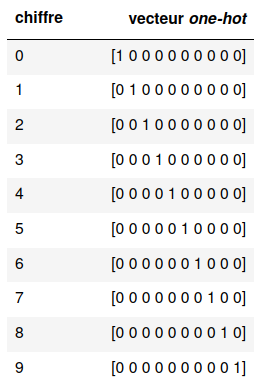
\includegraphics[width=1.1\textwidth]{images/oneHotCoded.png}
    \end{minipage}
    \begin{minipage}{.7\textwidth}
      Le codage {\em one-hot} des labels '0' à '9' donne un vecteur à 10 composantes, comme celui calculé par le réseau de neurones.
    \end{minipage}
  }
    
\end{frame}
%===============================================================================

%===============================================================================
\begin{frame}{1 - Réseau de neurones dense}

  \begin{tcolorbox}[title=Fonction d'erreur : {\em Cross entropy error}]  

    \begin{itemize}
    \item L'image traitée par le réseau $\leadsto$ vecteur $\hat{Y}$ de 10 \texttt{float} à comparer au vecteur $Y$ du codage {\em hot-one} du label de l'image.
    \item La fonction d'erreur (de perte) {\em cross entropy} est adaptée au codage {\em one-hot} : $e(Y,\hat{Y})=-\sum_i Y_i\ log(\hat{Y}_i)$\\
      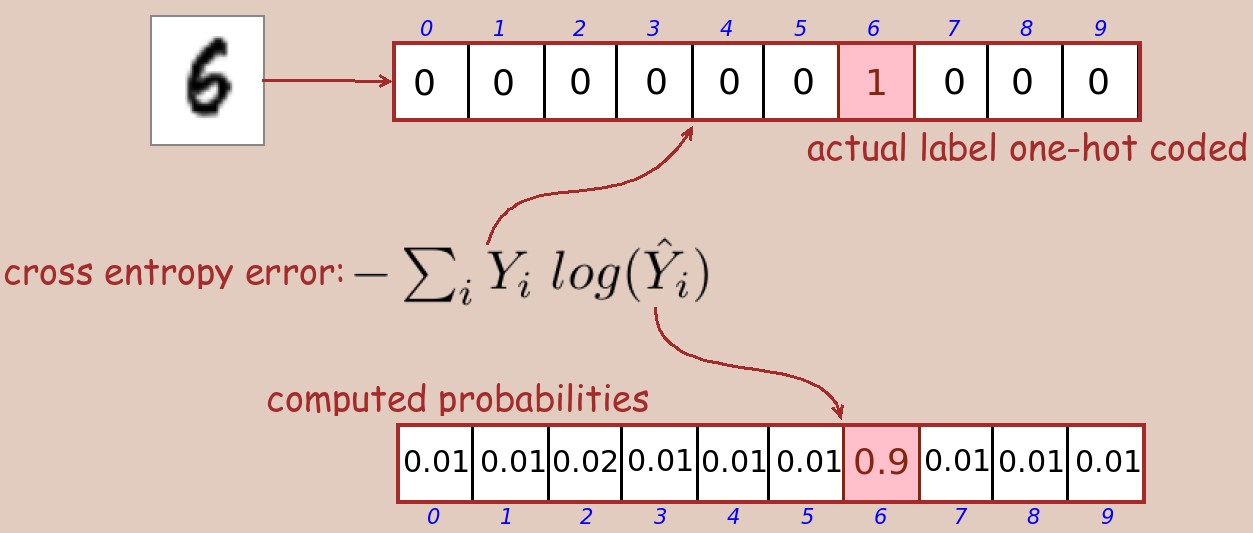
\includegraphics[width=.9\textwidth]{images/CrossEntropyError.png}
    \end{itemize}

  \end{tcolorbox}
  
\end{frame}
%===============================================================================

\subsection{Optimisation}

%===============================================================================
\begin{frame}{1 - Réseau de neurones dense}

  \begin{tcolorbox}[title=Optimisation et {\em Back Propagation}]  

    \begin{itemize}
        \visible<1->{\item Pendant la phase d'apprentissage un algorithme d'optimisation calcule le gradient de la fonction d'erreur 
            par rapport aux poids du réseau.}
        \visible<2->{\item L'algorithme de {\em Back Propagation} \textbf{modifie} les poids du réseau couche par couche grâce au gradient de la fonction d'erreur,
            en itérant de la dernière couche à la première couche. }
        \visible<3->{\item Exemples d'algorithme d'optimisation : 
        \begin{itemize}
        \item Descente de Gradient ({\em Gradient Descent (GD)})
        \item Descente de Gradient Stochastique ({\em Stochastic Gradient Descent (SGD)})
        \item {\em \href{https://arxiv.org/abs/1412.6980}{Adam}} (version améliorée de descente de gradient)...
        \end{itemize}

        {\small Le module \href{https://www.tensorflow.org/api_docs/python/tf/keras/optimizers}{tf.keras.optimizers}
          propose l'implémentation Python de plusieurs algorithmes d'optimisation.}}
      
    \end{itemize}
  \end{tcolorbox}
  
\end{frame}
%===============================================================================

\subsection{Back-propgation algorithm}

%===============================================================================
\begin{frame}{1 - Réseau de neurones dense}

  {\small Visualisation des itérations d'algorithmes de descente de gradient pour une fonction de perte ultra-simple à seulement 2 variables :}\\[2mm]
  \hspace*{25mm}\href{https://github.com/Jaewan-Yun/optimizer-visualization/blob/master/figures/movie9.gif}{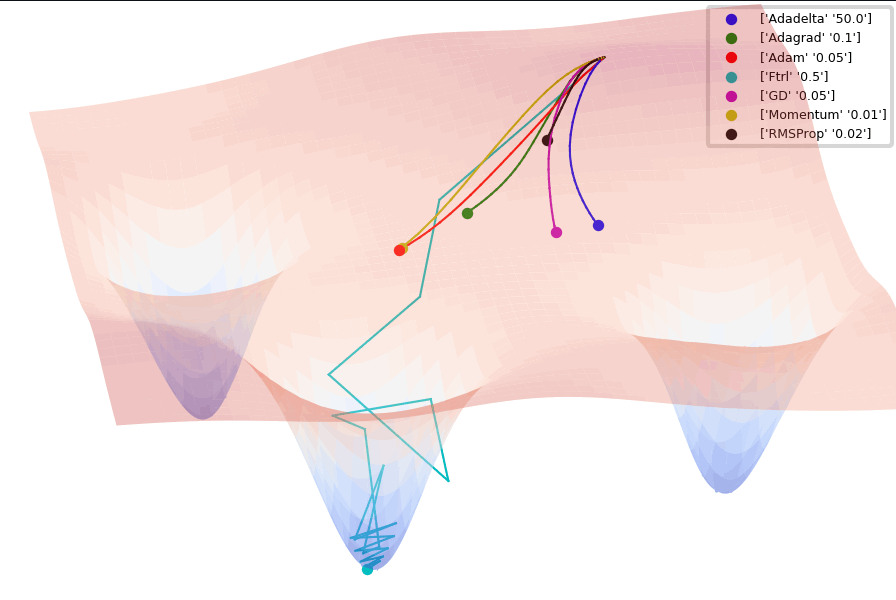
\includegraphics[width=.45\textwidth]{images/adam_plot3D_animated.png}}\\[-2mm]
  %\hspace*{8mm}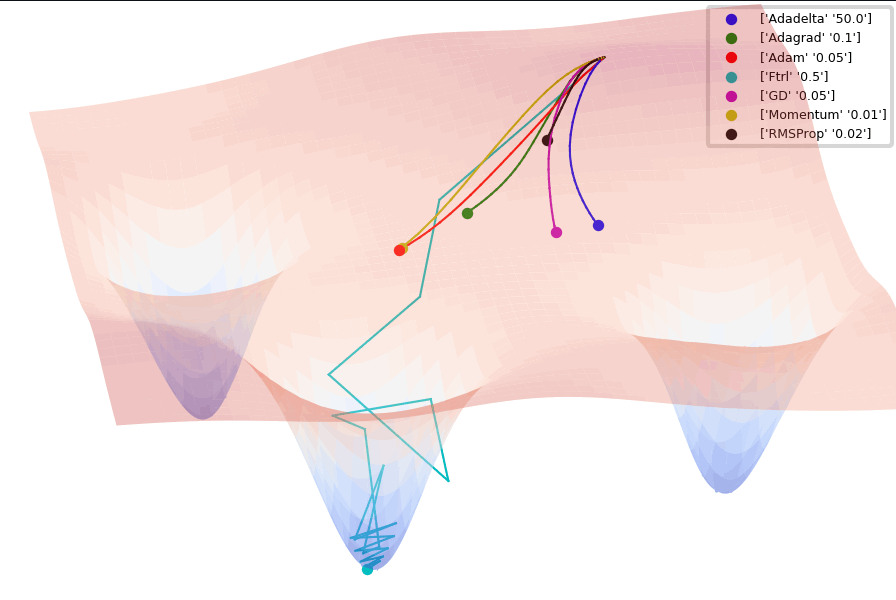
\includegraphics[width=.8\textwidth]{images/adam_plot3D_animated.png}\\[-2mm]
  %\animategraphics[width=.8\textwidth,controls]{10}{./images/Adam-plot3D/movie9/img_}{0}{114}
  \hspace*{25mm}{\tiny (source : \href{https://github.com/Jaewan-Yun/optimizer-visualization}{github.com/Jaewan-Yun/optimizer-visualization})}

  \medskip
  {\small Vidéo d'explication de l'algorithme de {\em back propagation} :}\\
  \hspace*{30mm}\href{https://www.3blue1brown.com/lessons/backpropagation}{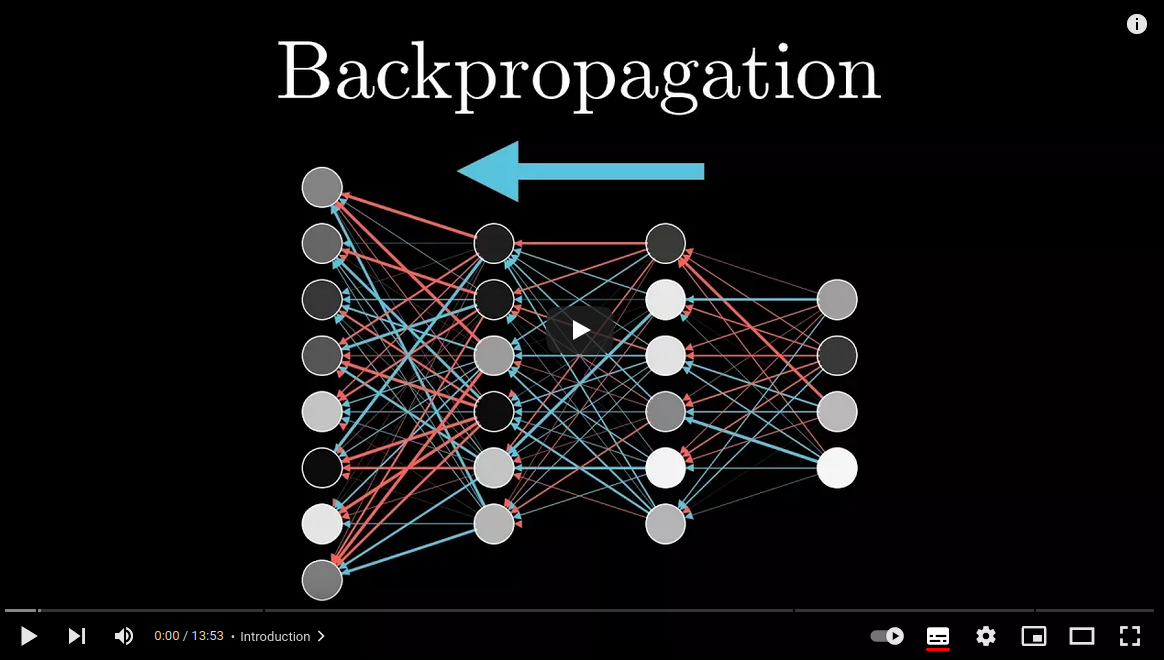
\includegraphics[width=.35\textwidth]{images/video-BackPropagation.png}}
\end{frame}
%===============================================================================

\subsection{Supervised learning}

%===============================================================================
\begin{frame}{}
  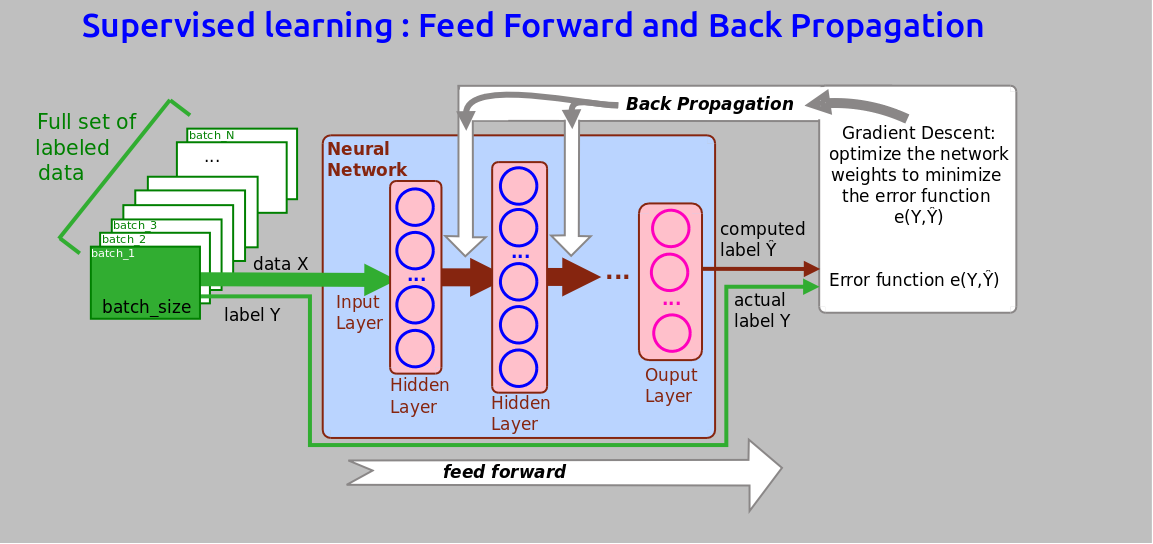
\includegraphics[width=1.2\textwidth]{./images/NetworkTraining.png}
  \vspace*{-3mm}\begin{itemize}
  \item Le jeu de données est découpé en (mini) {\bf batches} de taille \code{batch\_size}
  \item Après chaque {\em feed forward} l'algorithme de {\em Back Propagation} modifie les poids
    des neurones pour minimiser l'erreur $e$.
  \end{itemize}
\end{frame}
%===============================================================================

\subsection{Supervised learning}

%===============================================================================
\begin{frame}{}
  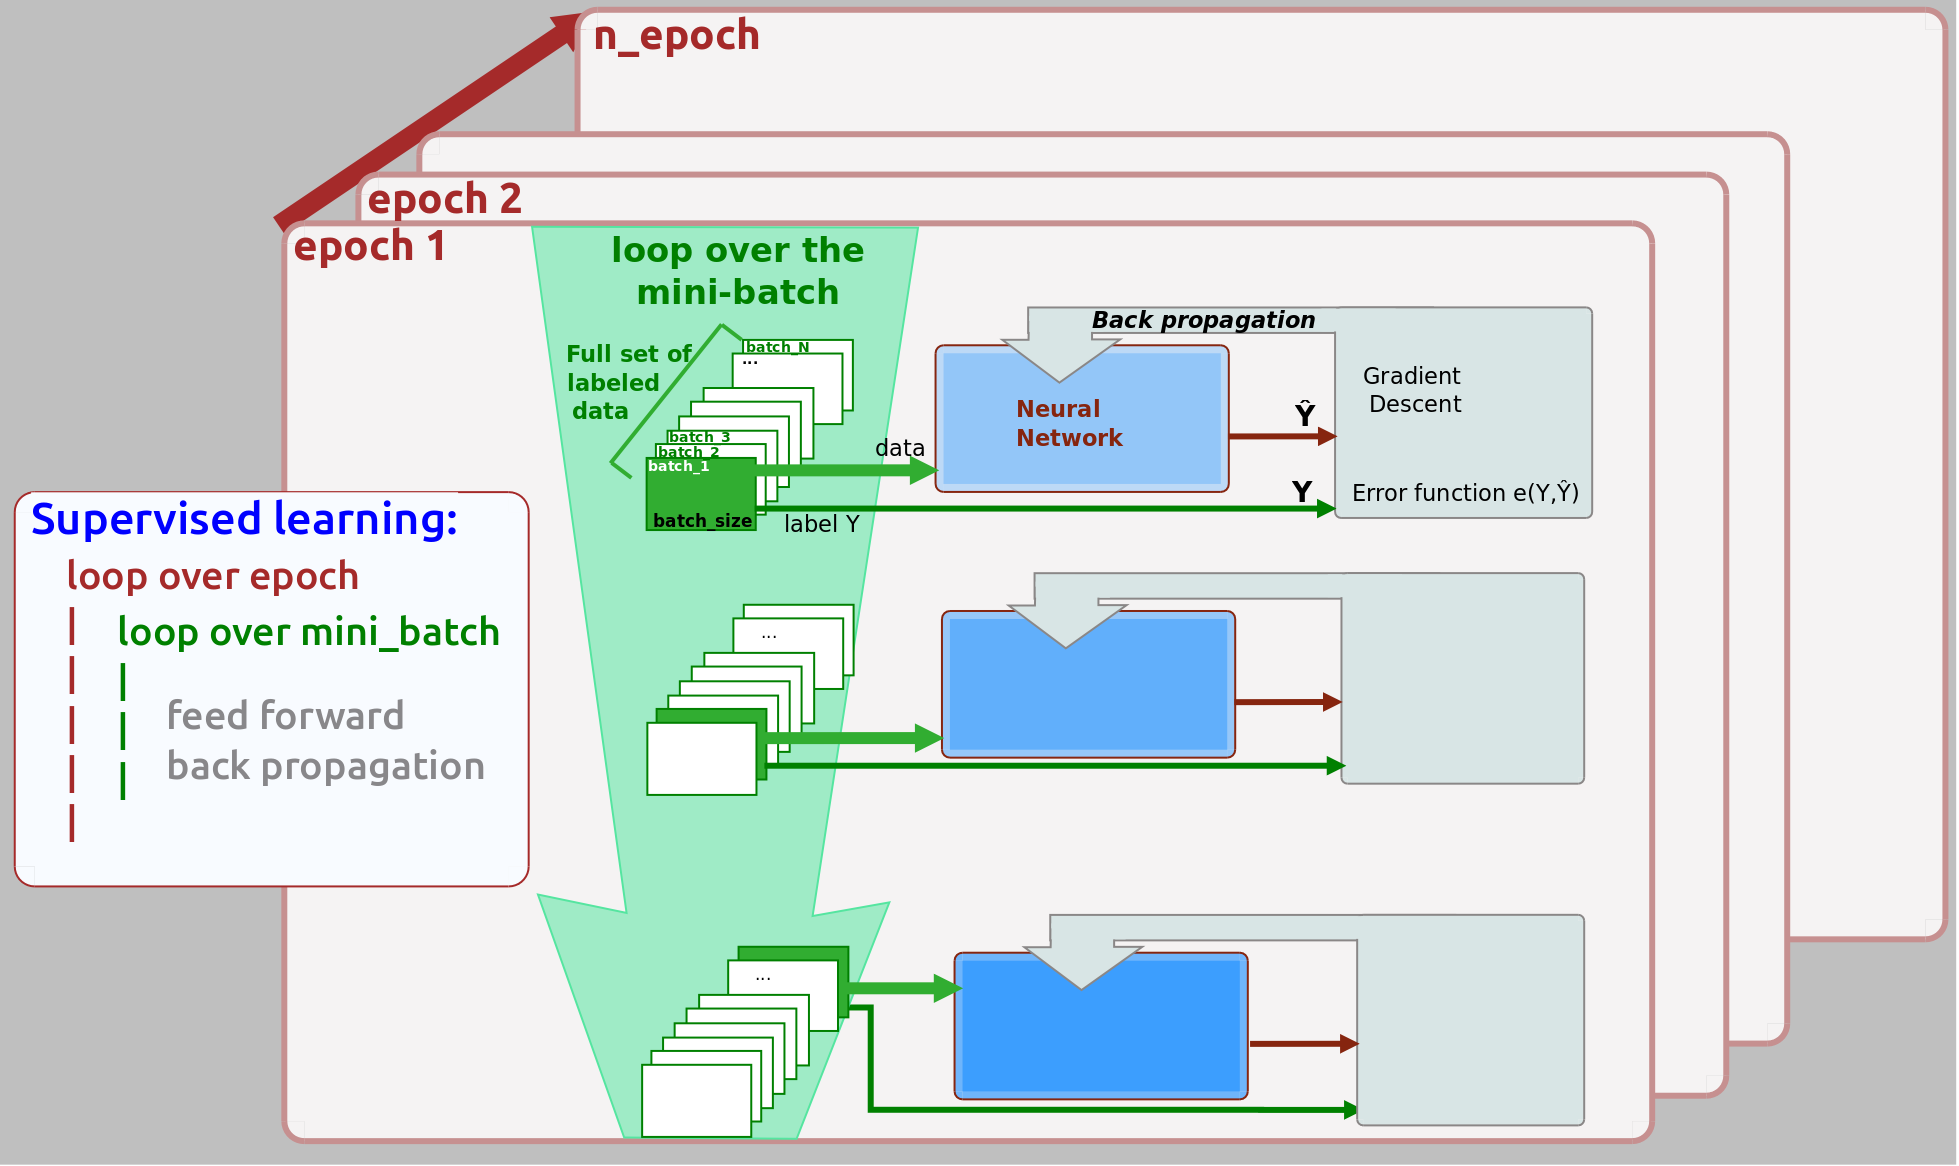
\includegraphics[width=\textwidth]{./images/NetworkTraining_2.png}
  \vspace*{-3mm}\begin{itemize}
  \item L'entraînement avec le jeu de données est répété \code{n\_epoch} fois,
  \item L'état du réseau à la fin de l'époque \code{n} sert d'état initial pour l'époque \code{n+1}.
  \end{itemize}
  
\end{frame}
%===============================================================================

 
\end{document}


To understand the difference between on-policy and off-policy, you need to understand that there are two phases of an RL algorithm:
the learning (or training) phase and the inference (or behaviour) phase (after the training phase).
The distinction between on-policy and off-policy algorithms only concerns the training phase.

There are mainly three ways to implement Reinforcement Learning. They are:

Value-based:
- learn the state-action value,
- acts by choosing the best action in the state.
- Estimates the policy by first estimating the associated value function
- Don't store any explicit policy, only a value function.
- The policy is here implicit and is derived from the value function (pick the action with the best value).
- Exploration is the key to value-based reinforcement learning
-> Q-Learning


Policy-based: directly learns the stochastic policy function that maps state to action. Act by sampling policy.
we explicitly build a representation of a policy $\pi(s,a)$ and keep it in memory during learning.

Model-based: refers to learning optimal behavior indirectly by learning a model of the environment by taking actions and observing the outcomes.

Model-based vs. Model-free

The problem we're often dealing with in RL is that whenever you are in state s
and make an action a you might not necessarily know the next state s'

that you'll end up in (the environment influences the agent).

In Model-based approach you either have an access to the model (environment) so you know the probability distribution over states that you end up in, or you first try to build a model (often - approximation) yourself. This might be useful because it allows you to do planning (you can "think" about making moves ahead without actually performing any actions).

In Model-free you're not given a model and you're not trying to explicitly figure out how it works. You just collect some experience and then derive (hopefully) optimal policy.



\section{Ressources}

%===============================================================================
\begin{frame}{Videos}

  \hspace*{-3mm}
  \href{https://youtu.be/trWrEWfhTVg}{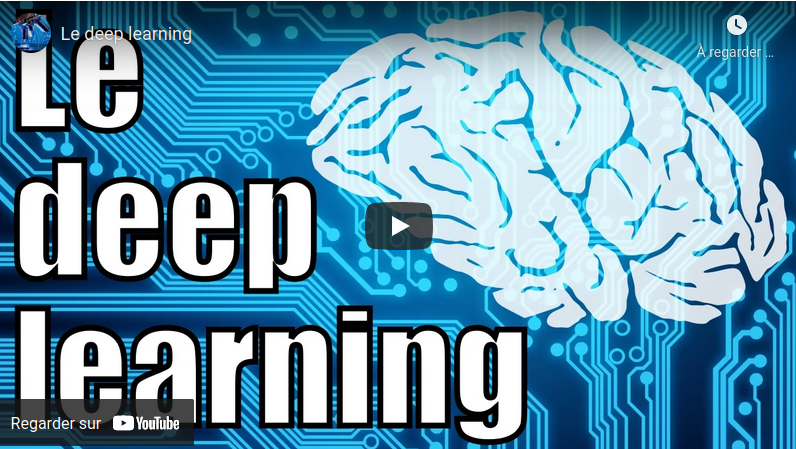
\includegraphics[width=.5\textwidth]{images/video-LeDeepLearning.png}}
  \hfill%
  \href{https://www.3blue1brown.com/lessons/neural-networks}{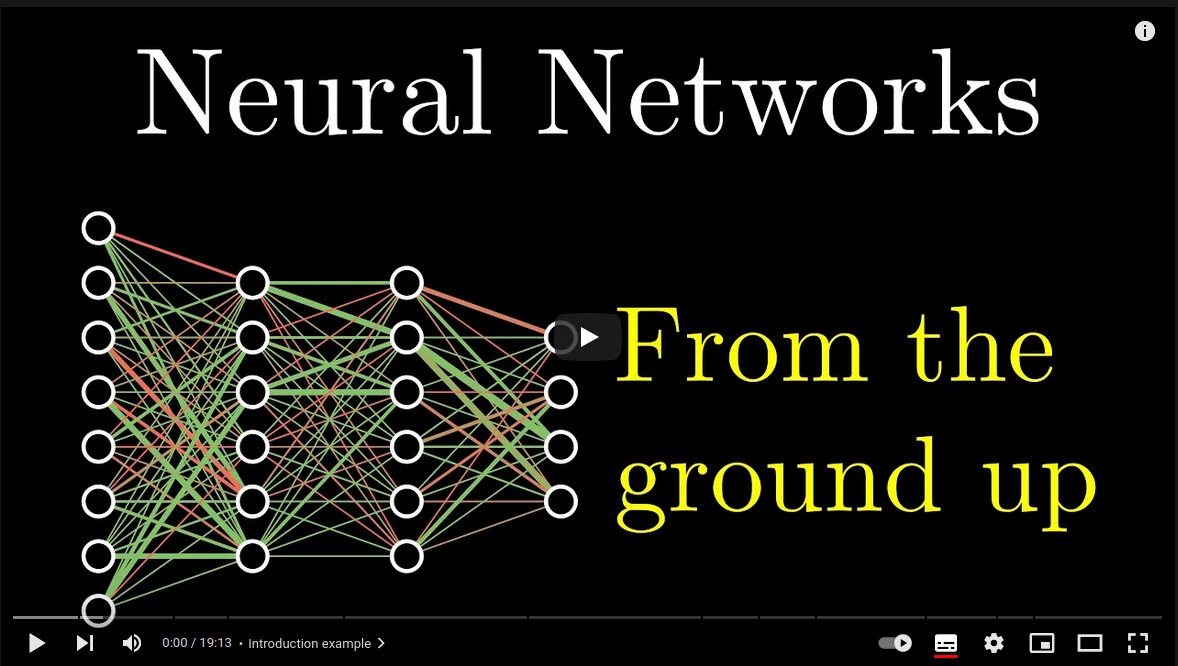
\includegraphics[width=.5\textwidth]{images/video-NeuralNetworks.png}}\\[-2mm]

  {\tiny\hspace*{-2mm}\href{run:./videos/Le deep learning - YouTube.webm}{1/ Local: "Le deep learning - YouTube.webm"}%
    \hfill%
    \href{run:./videos/But what is a neural network.webm}{2/ local : "But what is a neural network.webm"}}\\[2mm]
            
  \hspace*{-3mm}
  \href{https://www.3blue1brown.com/lessons/gradient-descent}{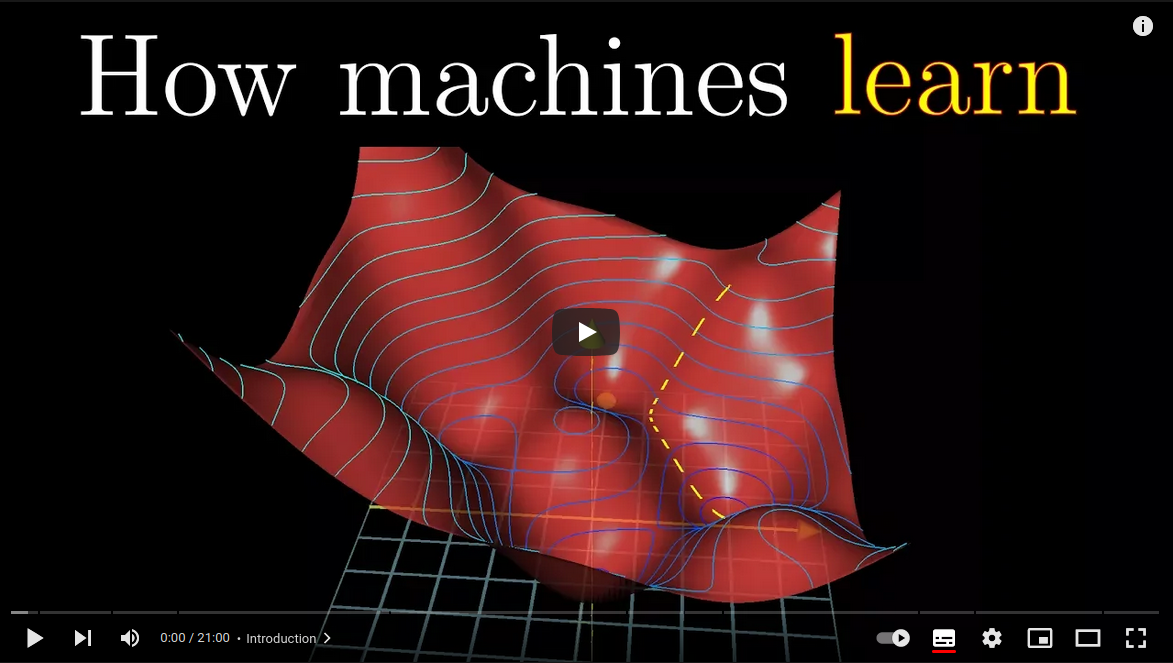
\includegraphics[width=.5\textwidth]{images/video-HowMachineLearn.png}}
  \hfill
  \href{https://www.3blue1brown.com/lessons/backpropagation}{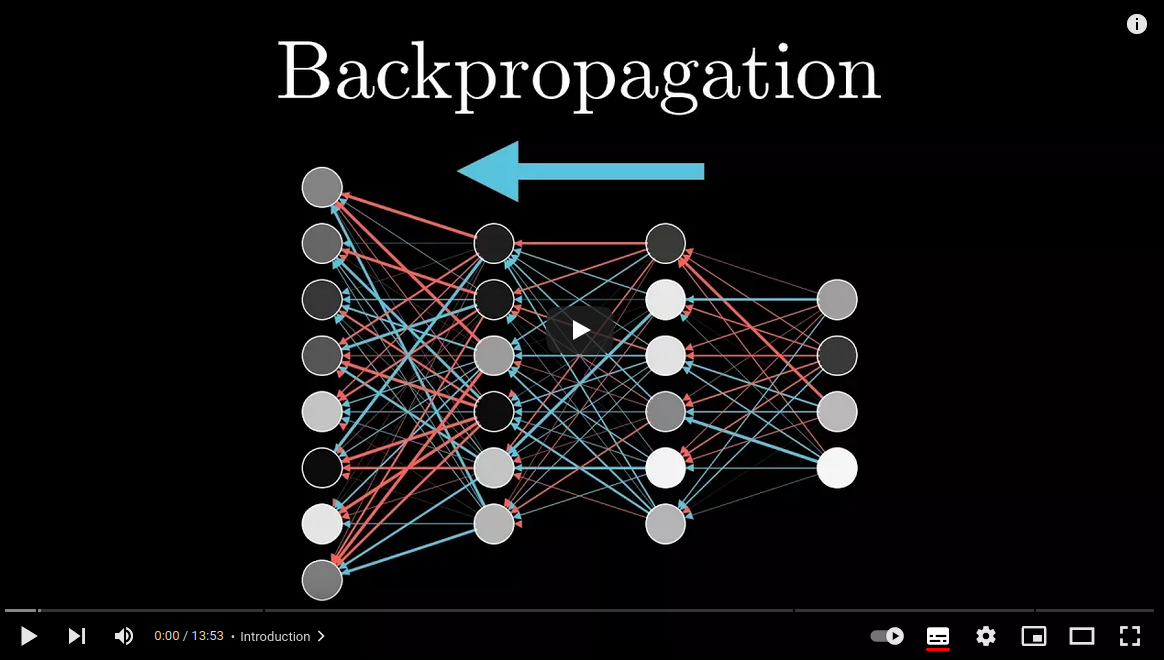
\includegraphics[width=.5\textwidth]{images/video-BackPropagation.png}}\\[-2mm]
  
  {\tiny\hspace*{-3mm}\href{run:./videos/Gradient descent how neural networks learn.webm}{3/ Local: "Gradient descent how neural networks learn.webm"}%
    \hfill%
    \href{run:./videos/What is backpropagation really doing .webm}{4/ Local: "What is backpropagation really doing .webm"}}\\[2mm]
  
\end{frame}
%===============================================================================

%===============================================================================

\end{document}

\begin{frame}{Biliographiesymbols for figures}

  \begin{figure}[hb]
    \begin{center}
        % PSTricks TeX macro
% Title: /home/jlc/work/IA-MachineLearning/1-ENSPIMA/2022-2023/course/Slides/images/NetworkTraining.dia
% Creator: Dia v0.97+git
% CreationDate: Thu Aug 25 14:32:05 2022
% For: jlc
% \usepackage{pstricks}
% The following commands are not supported in PSTricks at present
% We define them conditionally, so when they are implemented,
% this pstricks file will use them.
\ifx\setlinejoinmode\undefined
  \newcommand{\setlinejoinmode}[1]{}
\fi
\ifx\setlinecaps\undefined
  \newcommand{\setlinecaps}[1]{}
\fi
% This way define your own fonts mapping (for example with ifthen)
\ifx\setfont\undefined
  \newcommand{\setfont}[2]{}
\fi
\pspicture(9.016001,-19.069596)(61.087965,18.443030)
\psscalebox{1.000000 -1.000000}{
\newrgbcolor{dialinecolor}{0.000000 0.000000 0.000000}%
\psset{linecolor=dialinecolor}
\newrgbcolor{diafillcolor}{1.000000 1.000000 1.000000}%
\psset{fillcolor=diafillcolor}
\psset{linewidth=0.100000cm}
\psset{linestyle=solid}
\setlinejoinmode{0}
\newrgbcolor{diafillcolor}{1.000000 1.000000 1.000000}%
\psset{fillcolor=diafillcolor}
\newrgbcolor{dialinecolor}{0.000000 0.000000 0.000000}%
\psset{linecolor=dialinecolor}
\pspolygon[fillstyle=eofill,fillcolor=diafillcolor,linecolor=dialinecolor](9.066001,-14.397195)(61.037965,-14.397195)(61.037965,19.019596)(9.066001,19.019596)
\setfont{Helvetica}{0.800000}
\newrgbcolor{diafillcolor}{0.000000 0.000000 0.000000}%
\psset{fillcolor=diafillcolor}
\rput(35.051983,2.505263){\psscalebox{1 -1}{}}
\psset{linewidth=0.100000cm}
\psset{linestyle=solid}
\setlinejoinmode{0}
\setlinecaps{0}
\newrgbcolor{diafillcolor}{0.847059 0.898039 0.898039}%
\psset{fillcolor=diafillcolor}
\newrgbcolor{dialinecolor}{0.847059 0.898039 0.898039}%
\psset{linecolor=dialinecolor}
\pspolygon[fillstyle=eofill,fillcolor=diafillcolor,linecolor=dialinecolor](53.629356,-8.401769)(29.086115,-8.369035)(28.922539,-9.623118)(25.432918,-7.878307)(28.922539,-5.642769)(29.031589,-6.951377)(53.738407,-6.656962)
\psset{linewidth=0.100000cm}
\psset{linestyle=solid}
\setlinejoinmode{0}
\setlinecaps{0}
\newrgbcolor{diafillcolor}{1.000000 0.835294 0.650980}%
\psset{fillcolor=diafillcolor}
\newrgbcolor{dialinecolor}{0.909804 0.674510 0.364706}%
\psset{linecolor=dialinecolor}
\pscustom{
\newpath
\moveto(24.996725,-2.153147)
\curveto(24.396947,-6.624223)(31.212612,-7.005901)(40.372867,-7.060426)
\curveto(49.533121,-7.114951)(53.022742,-2.425773)(56.099290,-0.763688)
\curveto(59.175837,0.898397)(47.818490,2.999802)(48.526790,0.261040)
\curveto(49.235090,-2.477728)(45.601147,-3.002961)(44.241090,-3.341408)
\curveto(42.881032,-3.679856)(39.609512,-3.843432)(38.682582,-3.843432)
\curveto(37.755651,-3.843432)(31.158087,-4.388685)(31.703340,-2.480299)
\curveto(32.248593,-0.571912)(25.596504,2.317930)(24.996725,-2.153147)
\closepath
\fill[fillstyle=eofill,fillcolor=diafillcolor,linecolor=dialinecolor]}
\psset{linewidth=0.100000cm}
\psset{linestyle=solid}
\newrgbcolor{dialinecolor}{1.000000 0.835294 0.650980}%
\psset{linecolor=dialinecolor}
\psellipse*(53.018488,-0.826795)(6.369583,4.069450)
\newrgbcolor{dialinecolor}{1.000000 0.647059 0.000000}%
\psset{linecolor=dialinecolor}
\psellipse(53.018488,-0.826795)(6.369583,4.069450)
\setfont{Helvetica}{1.058333}
\newrgbcolor{diafillcolor}{0.000000 0.000000 0.000000}%
\psset{fillcolor=diafillcolor}
\rput[l](13.439621,-1.127595){\psscalebox{1 -1}{...}}
\setfont{Helvetica}{0.800000}
\newrgbcolor{diafillcolor}{0.000000 0.000000 0.000000}%
\psset{fillcolor=diafillcolor}
\rput[l](13.939621,0.872405){\psscalebox{1 -1}{}}
\setfont{Courier}{2.116667}
\newrgbcolor{diafillcolor}{0.000000 0.000000 0.000000}%
\psset{fillcolor=diafillcolor}
\rput[l](25.995921,-16.576895){\psscalebox{1 -1}{Supervised learning }}
\psset{linewidth=0.100000cm}
\psset{linestyle=solid}
\setlinejoinmode{0}
\newrgbcolor{diafillcolor}{0.886275 0.721569 0.631373}%
\psset{fillcolor=diafillcolor}
\pspolygon[fillstyle=eofill,fillcolor=diafillcolor](22.052921,-2.658395)(40.420307,-2.658395)(40.420307,13.107550)(22.052921,13.107550)
\newrgbcolor{diafillcolor}{0.886275 0.721569 0.631373}%
\psset{fillcolor=diafillcolor}
\pspolygon[fillstyle=eofill,fillcolor=diafillcolor](21.652921,-2.258395)(40.820307,-2.258395)(40.820307,12.707550)(21.652921,12.707550)
\newrgbcolor{dialinecolor}{0.886275 0.721569 0.631373}%
\psset{linecolor=dialinecolor}
\psclip{\pswedge[linestyle=none,fillstyle=none](22.052921,-2.258395){0.565685}{180.000000}{270.000000}}
\psellipse*(22.052921,-2.258395)(0.400000,0.400000)
\endpsclip
\newrgbcolor{dialinecolor}{0.525490 0.145098 0.058824}%
\psset{linecolor=dialinecolor}
\psclip{\pswedge[linestyle=none,fillstyle=none](22.052921,-2.258395){0.565685}{180.000000}{270.000000}}
\psellipse(22.052921,-2.258395)(0.400000,0.400000)
\endpsclip
\newrgbcolor{dialinecolor}{0.525490 0.145098 0.058824}%
\psset{linecolor=dialinecolor}
\psline(21.652921,-2.258395)(21.652921,12.707550)
\newrgbcolor{dialinecolor}{0.886275 0.721569 0.631373}%
\psset{linecolor=dialinecolor}
\psclip{\pswedge[linestyle=none,fillstyle=none](22.052921,12.707550){0.565685}{90.000000}{180.000000}}
\psellipse*(22.052921,12.707550)(0.400000,0.400000)
\endpsclip
\newrgbcolor{dialinecolor}{0.525490 0.145098 0.058824}%
\psset{linecolor=dialinecolor}
\psclip{\pswedge[linestyle=none,fillstyle=none](22.052921,12.707550){0.565685}{90.000000}{180.000000}}
\psellipse(22.052921,12.707550)(0.400000,0.400000)
\endpsclip
\newrgbcolor{dialinecolor}{0.525490 0.145098 0.058824}%
\psset{linecolor=dialinecolor}
\psline(22.052921,13.107550)(40.420307,13.107550)
\newrgbcolor{dialinecolor}{0.886275 0.721569 0.631373}%
\psset{linecolor=dialinecolor}
\psclip{\pswedge[linestyle=none,fillstyle=none](40.420307,12.707550){0.565685}{0.000000}{90.000000}}
\psellipse*(40.420307,12.707550)(0.400000,0.400000)
\endpsclip
\newrgbcolor{dialinecolor}{0.525490 0.145098 0.058824}%
\psset{linecolor=dialinecolor}
\psclip{\pswedge[linestyle=none,fillstyle=none](40.420307,12.707550){0.565685}{0.000000}{90.000000}}
\psellipse(40.420307,12.707550)(0.400000,0.400000)
\endpsclip
\newrgbcolor{dialinecolor}{0.525490 0.145098 0.058824}%
\psset{linecolor=dialinecolor}
\psline(40.820307,12.707550)(40.820307,-2.258395)
\newrgbcolor{dialinecolor}{0.886275 0.721569 0.631373}%
\psset{linecolor=dialinecolor}
\psclip{\pswedge[linestyle=none,fillstyle=none](40.420307,-2.258395){0.565685}{-90.000000}{0.000000}}
\psellipse*(40.420307,-2.258395)(0.400000,0.400000)
\endpsclip
\newrgbcolor{dialinecolor}{0.525490 0.145098 0.058824}%
\psset{linecolor=dialinecolor}
\psclip{\pswedge[linestyle=none,fillstyle=none](40.420307,-2.258395){0.565685}{-90.000000}{0.000000}}
\psellipse(40.420307,-2.258395)(0.400000,0.400000)
\endpsclip
\newrgbcolor{dialinecolor}{0.525490 0.145098 0.058824}%
\psset{linecolor=dialinecolor}
\psline(40.420307,-2.658395)(22.052921,-2.658395)
\setfont{Helvetica}{0.800000}
\newrgbcolor{diafillcolor}{0.000000 0.000000 0.000000}%
\psset{fillcolor=diafillcolor}
\rput(31.236614,5.418640){\psscalebox{1 -1}{}}
\psset{linewidth=0.200000cm}
\psset{linestyle=solid}
\setlinecaps{0}
\newrgbcolor{dialinecolor}{0.525490 0.145098 0.058824}%
\psset{linecolor=dialinecolor}
\psline(39.773088,4.280842)(48.333343,4.280842)
\psset{linewidth=0.200000cm}
\psset{linestyle=solid}
\setlinejoinmode{0}
\newrgbcolor{diafillcolor}{0.525490 0.145098 0.058824}%
\psset{fillcolor=diafillcolor}
\newrgbcolor{dialinecolor}{0.525490 0.145098 0.058824}%
\psset{linecolor=dialinecolor}
\pspolygon[fillstyle=eofill,fillcolor=diafillcolor,linecolor=dialinecolor](48.333343,4.530842)(48.833343,4.280842)(48.333343,4.030842)
\psset{linewidth=0.100000cm}
\psset{linestyle=solid}
\setlinejoinmode{0}
\setlinecaps{0}
\newrgbcolor{diafillcolor}{0.000000 0.501961 0.000000}%
\psset{fillcolor=diafillcolor}
\newrgbcolor{dialinecolor}{0.000000 0.501961 0.000000}%
\psset{linecolor=dialinecolor}
\pspolygon[fillstyle=eofill,fillcolor=diafillcolor,linecolor=dialinecolor](10.531621,-12.627595)(16.939617,-12.627595)(16.939617,6.530583)(10.531621,6.530583)
\psset{linewidth=0.200000cm}
\psset{linestyle=solid}
\setlinejoinmode{0}
\setlinecaps{0}
\newrgbcolor{dialinecolor}{0.000000 0.501961 0.000000}%
\psset{linecolor=dialinecolor}
\psline(17.010088,5.113984)(21.043046,5.113984)(21.043046,13.538529)(41.383446,13.538529)(41.383446,5.425873)(48.442393,5.425873)
\psset{linewidth=0.200000cm}
\psset{linestyle=solid}
\setlinejoinmode{0}
\newrgbcolor{diafillcolor}{0.000000 0.501961 0.000000}%
\psset{fillcolor=diafillcolor}
\newrgbcolor{dialinecolor}{0.000000 0.501961 0.000000}%
\psset{linecolor=dialinecolor}
\pspolygon[fillstyle=eofill,fillcolor=diafillcolor,linecolor=dialinecolor](48.442393,5.675873)(48.942393,5.425873)(48.442393,5.175873)
\psset{linewidth=0.100000cm}
\psset{linestyle=solid}
\newrgbcolor{dialinecolor}{0.956863 0.592157 0.592157}%
\psset{linecolor=dialinecolor}
\psellipse*(53.602834,4.717731)(4.626160,2.270403)
\newrgbcolor{dialinecolor}{1.000000 0.752941 0.796078}%
\psset{linecolor=dialinecolor}
\psellipse(53.602834,4.717731)(4.626160,2.270403)
\psset{linewidth=0.100000cm}
\psset{linestyle=solid}
\setlinejoinmode{1}
\setlinecaps{0}
\newrgbcolor{diafillcolor}{1.000000 0.752941 0.796078}%
\psset{fillcolor=diafillcolor}
\pspolygon[fillstyle=eofill,fillcolor=diafillcolor](36.927621,0.485808)(39.087286,0.485808)(39.087286,7.546701)(36.927621,7.546701)
\newrgbcolor{diafillcolor}{1.000000 0.752941 0.796078}%
\psset{fillcolor=diafillcolor}
\pspolygon[fillstyle=eofill,fillcolor=diafillcolor](36.427621,0.985808)(39.587286,0.985808)(39.587286,7.046701)(36.427621,7.046701)
\newrgbcolor{dialinecolor}{1.000000 0.752941 0.796078}%
\psset{linecolor=dialinecolor}
\psclip{\pswedge[linestyle=none,fillstyle=none](36.927621,0.985808){0.707107}{180.000000}{270.000000}}
\psellipse*(36.927621,0.985808)(0.500000,0.500000)
\endpsclip
\newrgbcolor{dialinecolor}{0.525490 0.145098 0.058824}%
\psset{linecolor=dialinecolor}
\psclip{\pswedge[linestyle=none,fillstyle=none](36.927621,0.985808){0.707107}{180.000000}{270.000000}}
\psellipse(36.927621,0.985808)(0.500000,0.500000)
\endpsclip
\newrgbcolor{dialinecolor}{0.525490 0.145098 0.058824}%
\psset{linecolor=dialinecolor}
\psline(36.427621,0.985808)(36.427621,7.046701)
\newrgbcolor{dialinecolor}{1.000000 0.752941 0.796078}%
\psset{linecolor=dialinecolor}
\psclip{\pswedge[linestyle=none,fillstyle=none](36.927621,7.046701){0.707107}{90.000000}{180.000000}}
\psellipse*(36.927621,7.046701)(0.500000,0.500000)
\endpsclip
\newrgbcolor{dialinecolor}{0.525490 0.145098 0.058824}%
\psset{linecolor=dialinecolor}
\psclip{\pswedge[linestyle=none,fillstyle=none](36.927621,7.046701){0.707107}{90.000000}{180.000000}}
\psellipse(36.927621,7.046701)(0.500000,0.500000)
\endpsclip
\newrgbcolor{dialinecolor}{0.525490 0.145098 0.058824}%
\psset{linecolor=dialinecolor}
\psline(36.927621,7.546701)(39.087286,7.546701)
\newrgbcolor{dialinecolor}{1.000000 0.752941 0.796078}%
\psset{linecolor=dialinecolor}
\psclip{\pswedge[linestyle=none,fillstyle=none](39.087286,7.046701){0.707107}{0.000000}{90.000000}}
\psellipse*(39.087286,7.046701)(0.500000,0.500000)
\endpsclip
\newrgbcolor{dialinecolor}{0.525490 0.145098 0.058824}%
\psset{linecolor=dialinecolor}
\psclip{\pswedge[linestyle=none,fillstyle=none](39.087286,7.046701){0.707107}{0.000000}{90.000000}}
\psellipse(39.087286,7.046701)(0.500000,0.500000)
\endpsclip
\newrgbcolor{dialinecolor}{0.525490 0.145098 0.058824}%
\psset{linecolor=dialinecolor}
\psline(39.587286,7.046701)(39.587286,0.985808)
\newrgbcolor{dialinecolor}{1.000000 0.752941 0.796078}%
\psset{linecolor=dialinecolor}
\psclip{\pswedge[linestyle=none,fillstyle=none](39.087286,0.985808){0.707107}{-90.000000}{0.000000}}
\psellipse*(39.087286,0.985808)(0.500000,0.500000)
\endpsclip
\newrgbcolor{dialinecolor}{0.525490 0.145098 0.058824}%
\psset{linecolor=dialinecolor}
\psclip{\pswedge[linestyle=none,fillstyle=none](39.087286,0.985808){0.707107}{-90.000000}{0.000000}}
\psellipse(39.087286,0.985808)(0.500000,0.500000)
\endpsclip
\newrgbcolor{dialinecolor}{0.525490 0.145098 0.058824}%
\psset{linecolor=dialinecolor}
\psline(39.087286,0.485808)(36.927621,0.485808)
\psset{linewidth=0.400000cm}
\psset{linestyle=solid}
\setlinecaps{0}
\newrgbcolor{dialinecolor}{0.000000 0.501961 0.000000}%
\psset{linecolor=dialinecolor}
\psline(16.920208,4.429032)(23.576121,4.432411)
\psset{linewidth=0.400000cm}
\psset{linestyle=solid}
\setlinejoinmode{0}
\newrgbcolor{diafillcolor}{0.000000 0.501961 0.000000}%
\psset{fillcolor=diafillcolor}
\newrgbcolor{dialinecolor}{0.000000 0.501961 0.000000}%
\psset{linecolor=dialinecolor}
\pspolygon[fillstyle=eofill,fillcolor=diafillcolor,linecolor=dialinecolor](23.575994,4.682411)(24.076121,4.432664)(23.576248,4.182411)
\setfont{Helvetica}{1.058333}
\newrgbcolor{diafillcolor}{0.525490 0.145098 0.058824}%
\psset{fillcolor=diafillcolor}
\rput[l](24.854121,11.711705){\psscalebox{1 -1}{Hidden }}
\setfont{Helvetica}{1.058333}
\newrgbcolor{diafillcolor}{0.525490 0.145098 0.058824}%
\psset{fillcolor=diafillcolor}
\rput[l](24.854121,12.770038){\psscalebox{1 -1}{Layer}}
\setfont{Helvetica}{1.058333}
\newrgbcolor{diafillcolor}{0.525490 0.145098 0.058824}%
\psset{fillcolor=diafillcolor}
\rput[l](21.915521,5.986015){\psscalebox{1 -1}{Input}}
\setfont{Helvetica}{1.058333}
\newrgbcolor{diafillcolor}{0.525490 0.145098 0.058824}%
\psset{fillcolor=diafillcolor}
\rput[l](21.915521,7.044348){\psscalebox{1 -1}{Layer}}
\setfont{Helvetica}{1.058333}
\newrgbcolor{diafillcolor}{0.525490 0.145098 0.058824}%
\psset{fillcolor=diafillcolor}
\rput[l](36.709321,8.578875){\psscalebox{1 -1}{Ouput}}
\setfont{Helvetica}{1.058333}
\newrgbcolor{diafillcolor}{0.525490 0.145098 0.058824}%
\psset{fillcolor=diafillcolor}
\rput[l](36.709321,9.637208){\psscalebox{1 -1}{Layer}}
\setfont{Helvetica}{1.058333}
\newrgbcolor{diafillcolor}{0.525490 0.145098 0.058824}%
\psset{fillcolor=diafillcolor}
\rput[l](29.642721,11.752105){\psscalebox{1 -1}{Hidden }}
\setfont{Helvetica}{1.058333}
\newrgbcolor{diafillcolor}{0.525490 0.145098 0.058824}%
\psset{fillcolor=diafillcolor}
\rput[l](29.642721,12.810438){\psscalebox{1 -1}{Layer}}
\psset{linewidth=0.100000cm}
\psset{linestyle=solid}
\setlinejoinmode{0}
\setlinecaps{0}
\newrgbcolor{diafillcolor}{1.000000 0.835294 0.650980}%
\psset{fillcolor=diafillcolor}
\newrgbcolor{dialinecolor}{1.000000 0.835294 0.650980}%
\psset{linecolor=dialinecolor}
\pspolygon[fillstyle=eofill,fillcolor=diafillcolor,linecolor=dialinecolor](31.182721,-3.376415)(31.199821,-2.396215)(31.796621,-2.384795)(30.816821,-1.404975)(29.813421,-2.420205)(30.498121,-2.432015)(30.498121,-3.376415)
\psset{linewidth=0.100000cm}
\psset{linestyle=solid}
\setlinejoinmode{0}
\setlinecaps{0}
\newrgbcolor{diafillcolor}{1.000000 0.835294 0.650980}%
\psset{fillcolor=diafillcolor}
\newrgbcolor{dialinecolor}{1.000000 0.835294 0.650980}%
\psset{linecolor=dialinecolor}
\pspolygon[fillstyle=eofill,fillcolor=diafillcolor,linecolor=dialinecolor](26.371521,-2.887185)(26.329521,-1.345625)(26.955221,-1.333825)(25.975421,-0.354005)(24.972021,-1.369235)(25.656621,-1.381045)(25.539021,-2.827725)
\setfont{Courier}{1.763889}
\newrgbcolor{diafillcolor}{0.000000 0.000000 0.000000}%
\psset{fillcolor=diafillcolor}
\rput[l](30.357421,-13.179995){\psscalebox{1 -1}{one epoch}}
\setfont{Helvetica}{1.058333}
\newrgbcolor{diafillcolor}{0.000000 0.000000 0.000000}%
\psset{fillcolor=diafillcolor}
\rput[l](9.926471,-13.211395){\psscalebox{1 -1}{input data with labels}}
\psset{linewidth=0.300000cm}
\psset{linestyle=solid}
\setlinecaps{0}
\newrgbcolor{dialinecolor}{0.525490 0.145098 0.058824}%
\psset{linecolor=dialinecolor}
\psline(27.708392,4.432766)(28.426928,4.429421)
\psset{linewidth=0.300000cm}
\psset{linestyle=solid}
\setlinejoinmode{0}
\newrgbcolor{diafillcolor}{0.525490 0.145098 0.058824}%
\psset{fillcolor=diafillcolor}
\newrgbcolor{dialinecolor}{0.525490 0.145098 0.058824}%
\psset{linecolor=dialinecolor}
\pspolygon[fillstyle=eofill,fillcolor=diafillcolor,linecolor=dialinecolor](28.428092,4.679418)(28.926922,4.427093)(28.425764,4.179424)
\psset{linewidth=0.100000cm}
\psset{linestyle=solid}
\setlinejoinmode{1}
\setlinecaps{0}
\newrgbcolor{diafillcolor}{1.000000 0.752941 0.796078}%
\psset{fillcolor=diafillcolor}
\pspolygon[fillstyle=eofill,fillcolor=diafillcolor](24.576121,-0.392155)(27.408392,-0.392155)(27.408392,9.257687)(24.576121,9.257687)
\newrgbcolor{diafillcolor}{1.000000 0.752941 0.796078}%
\psset{fillcolor=diafillcolor}
\pspolygon[fillstyle=eofill,fillcolor=diafillcolor](24.276121,-0.092155)(27.708392,-0.092155)(27.708392,8.957687)(24.276121,8.957687)
\newrgbcolor{dialinecolor}{1.000000 0.752941 0.796078}%
\psset{linecolor=dialinecolor}
\psclip{\pswedge[linestyle=none,fillstyle=none](24.576121,-0.092155){0.424264}{180.000000}{270.000000}}
\psellipse*(24.576121,-0.092155)(0.300000,0.300000)
\endpsclip
\newrgbcolor{dialinecolor}{0.525490 0.145098 0.058824}%
\psset{linecolor=dialinecolor}
\psclip{\pswedge[linestyle=none,fillstyle=none](24.576121,-0.092155){0.424264}{180.000000}{270.000000}}
\psellipse(24.576121,-0.092155)(0.300000,0.300000)
\endpsclip
\newrgbcolor{dialinecolor}{0.525490 0.145098 0.058824}%
\psset{linecolor=dialinecolor}
\psline(24.276121,-0.092155)(24.276121,8.957687)
\newrgbcolor{dialinecolor}{1.000000 0.752941 0.796078}%
\psset{linecolor=dialinecolor}
\psclip{\pswedge[linestyle=none,fillstyle=none](24.576121,8.957687){0.424264}{90.000000}{180.000000}}
\psellipse*(24.576121,8.957687)(0.300000,0.300000)
\endpsclip
\newrgbcolor{dialinecolor}{0.525490 0.145098 0.058824}%
\psset{linecolor=dialinecolor}
\psclip{\pswedge[linestyle=none,fillstyle=none](24.576121,8.957687){0.424264}{90.000000}{180.000000}}
\psellipse(24.576121,8.957687)(0.300000,0.300000)
\endpsclip
\newrgbcolor{dialinecolor}{0.525490 0.145098 0.058824}%
\psset{linecolor=dialinecolor}
\psline(24.576121,9.257687)(27.408392,9.257687)
\newrgbcolor{dialinecolor}{1.000000 0.752941 0.796078}%
\psset{linecolor=dialinecolor}
\psclip{\pswedge[linestyle=none,fillstyle=none](27.408392,8.957687){0.424264}{0.000000}{90.000000}}
\psellipse*(27.408392,8.957687)(0.300000,0.300000)
\endpsclip
\newrgbcolor{dialinecolor}{0.525490 0.145098 0.058824}%
\psset{linecolor=dialinecolor}
\psclip{\pswedge[linestyle=none,fillstyle=none](27.408392,8.957687){0.424264}{0.000000}{90.000000}}
\psellipse(27.408392,8.957687)(0.300000,0.300000)
\endpsclip
\newrgbcolor{dialinecolor}{0.525490 0.145098 0.058824}%
\psset{linecolor=dialinecolor}
\psline(27.708392,8.957687)(27.708392,-0.092155)
\newrgbcolor{dialinecolor}{1.000000 0.752941 0.796078}%
\psset{linecolor=dialinecolor}
\psclip{\pswedge[linestyle=none,fillstyle=none](27.408392,-0.092155){0.424264}{-90.000000}{0.000000}}
\psellipse*(27.408392,-0.092155)(0.300000,0.300000)
\endpsclip
\newrgbcolor{dialinecolor}{0.525490 0.145098 0.058824}%
\psset{linecolor=dialinecolor}
\psclip{\pswedge[linestyle=none,fillstyle=none](27.408392,-0.092155){0.424264}{-90.000000}{0.000000}}
\psellipse(27.408392,-0.092155)(0.300000,0.300000)
\endpsclip
\newrgbcolor{dialinecolor}{0.525490 0.145098 0.058824}%
\psset{linecolor=dialinecolor}
\psline(27.408392,-0.392155)(24.576121,-0.392155)
\psset{linewidth=0.150000cm}
\psset{linestyle=solid}
\newrgbcolor{dialinecolor}{1.000000 0.752941 0.796078}%
\psset{linecolor=dialinecolor}
\psellipse*(25.992190,0.918257)(0.914470,0.914470)
\newrgbcolor{dialinecolor}{0.000000 0.000000 1.000000}%
\psset{linecolor=dialinecolor}
\psellipse(25.992190,0.918257)(0.914470,0.914470)
\psset{linewidth=0.150000cm}
\psset{linestyle=solid}
\newrgbcolor{dialinecolor}{1.000000 0.752941 0.796078}%
\psset{linecolor=dialinecolor}
\psellipse*(25.992190,3.095425)(0.914470,0.914470)
\newrgbcolor{dialinecolor}{0.000000 0.000000 1.000000}%
\psset{linecolor=dialinecolor}
\psellipse(25.992190,3.095425)(0.914470,0.914470)
\setfont{Helvetica-Bold}{1.058333}
\newrgbcolor{diafillcolor}{0.000000 0.000000 1.000000}%
\psset{fillcolor=diafillcolor}
\rput[l](25.604721,4.587615){\psscalebox{1 -1}{...}}
\psset{linewidth=0.150000cm}
\psset{linestyle=solid}
\newrgbcolor{dialinecolor}{1.000000 0.752941 0.796078}%
\psset{linecolor=dialinecolor}
\psellipse*(25.992190,5.807305)(0.914470,0.914470)
\newrgbcolor{dialinecolor}{0.000000 0.000000 1.000000}%
\psset{linecolor=dialinecolor}
\psellipse(25.992190,5.807305)(0.914470,0.914470)
\psset{linewidth=0.150000cm}
\psset{linestyle=solid}
\newrgbcolor{dialinecolor}{1.000000 0.752941 0.796078}%
\psset{linecolor=dialinecolor}
\psellipse*(25.992190,8.003735)(0.914470,0.914470)
\newrgbcolor{dialinecolor}{0.000000 0.000000 1.000000}%
\psset{linecolor=dialinecolor}
\psellipse(25.992190,8.003735)(0.914470,0.914470)
\setfont{Helvetica}{1.058333}
\newrgbcolor{diafillcolor}{0.000000 0.000000 0.000000}%
\psset{fillcolor=diafillcolor}
\rput(53.509199,4.551263){\psscalebox{1 -1}{Cost function}}
\setfont{Helvetica}{1.058333}
\newrgbcolor{diafillcolor}{0.000000 0.000000 0.000000}%
\psset{fillcolor=diafillcolor}
\rput(53.509199,5.609597){\psscalebox{1 -1}{-> e: error}}
\setfont{Helvetica}{1.058333}
\newrgbcolor{diafillcolor}{0.000000 0.000000 0.000000}%
\psset{fillcolor=diafillcolor}
\rput(53.509199,6.667930){\psscalebox{1 -1}{}}
\psset{linewidth=0.150000cm}
\psset{linestyle=solid}
\newrgbcolor{dialinecolor}{1.000000 0.752941 0.796078}%
\psset{linecolor=dialinecolor}
\psellipse*(38.022090,1.738266)(0.914470,0.914470)
\newrgbcolor{dialinecolor}{1.000000 0.000000 0.741176}%
\psset{linecolor=dialinecolor}
\psellipse(38.022090,1.738266)(0.914470,0.914470)
\psset{linewidth=0.150000cm}
\psset{linestyle=solid}
\newrgbcolor{dialinecolor}{1.000000 0.752941 0.796078}%
\psset{linecolor=dialinecolor}
\psellipse*(37.962690,3.938285)(0.914470,0.914470)
\newrgbcolor{dialinecolor}{1.000000 0.000000 0.741176}%
\psset{linecolor=dialinecolor}
\psellipse(37.962690,3.938285)(0.914470,0.914470)
\psset{linewidth=0.150000cm}
\psset{linestyle=solid}
\newrgbcolor{dialinecolor}{1.000000 0.752941 0.796078}%
\psset{linecolor=dialinecolor}
\psellipse*(38.039990,6.206685)(0.914470,0.914470)
\newrgbcolor{dialinecolor}{1.000000 0.000000 0.741176}%
\psset{linecolor=dialinecolor}
\psellipse(38.039990,6.206685)(0.914470,0.914470)
\setfont{Helvetica-Bold}{1.411111}
\newrgbcolor{diafillcolor}{0.525490 0.145098 0.058824}%
\psset{fillcolor=diafillcolor}
\rput[l](34.713721,4.656335){\psscalebox{1 -1}{...}}
\setfont{Helvetica-Bold}{1.058333}
\newrgbcolor{diafillcolor}{0.525490 0.145098 0.058824}%
\psset{fillcolor=diafillcolor}
\rput[l](33.004821,-1.595255){\psscalebox{1 -1}{Neural Network}}
\pscustom{\code{gsave
/pix 111 string def
/grays 37 string def
/npixls 0 def
/rgbindx 0 def
28.346000 28.346000 scale
19.509021 5.405975 translate
1.056856 1.371056 scale
37 48 8
[37 0 0 48 0 0]
{currentfile pix readhexstring pop}
false 3 colorimage
ffffffffffffffffffffffffffffffffffffffffffffffffffffffffffffffffffffffffffffffffffffffffffffffffffffffffffffffffffffffffffffffffffffffffffffffffffffffffffffffffffffffffffffffffffffffffffffffffffffffffffffffffffffffffffffff
ffffffffffffffffffffffffffffffffffffffffffffffffffffffffffffffffffffffffffffffffffffffffffffffffffffffffffffffffffffffffffffffffffffffffffffffffffffffffffffffffffffffffffffffffffffffffffffffffffffffffffffffffffffffffffffff
ffffffffffffffffffffffffffffffffffffffffffffffffffffffffffffffffffffffffffffffffffffffffffffffffffffffffffffffffffffffffffffffffffffffffffffffffffffffffffffffffffffffffffffffffffffffffffffffffffffffffffffffffffffffffffffff
ffffffffffffffffffffffffffffffffffffffffffffffffffffffffffffffffffffffffffffffffffffffffffffffffffffffffffffffffffffffffffffffffffffffffffffffffffffffffffffffffffffffffffffffffffffffffffffffffffffffffffffffffffffffffffffff
ffffffffffffffffffffffffffffffffffffffffffffffffffffffffffffffffffffffffffffffffffffffffffffffffffffffffffffffffffffffffffffffffffffffffffffffffffffffffffffffffffffffffffffffffffffffffffffffffffffffffffffffffffffffffffffff
ffffffffffffffffffffffffffffffffffffffffffffffffffffffffffffffffffffffffffffffffffffffffffffffffffffffffffffffffffffffffffffffffffffffffffffffffffffffffffffffffffffffffffffffffffffffffffffffffffffffffffffffffffffffffffffff
ffffffffffffffffffffffffffffffffffffffffffffffffffffffffffffffffffffffffffffffffffffffffffffffffffffffffffffffffffffffffffffffffffffffffffffffffffffffffffffffffffffffffffffffffffffffffffffffffffffffffffffffffffffffffffffff
ffffffffffffffffffffffffffffffffffffffffffffffffffffffffffffffffffffffffffffffffffffffffffffffffffffffffffffffffffffffffffffffffffffffffffffffffffffffffffffffffffffffffffffffffffffffffffffffffffffffffffffffffffffffffffffff
ffffffffffffffffffffffffe7e7e78d8d8d8e8e8e969696a0a0a0a8a8a8abababa7a7a7a0a0a09898989090908b8b8bc2c2c2ffffffffffffffffffffffffffffffffffffffffffffffffffffffffffffdbdbdb8c8c8c9292929a9a9aa2a2a2a9a9a9a5a5a59b9b9b9292929d9d9d
ffffffffffffffffffffffffb4b4b41616160707070000000000000000000000000000000000000000000303031414147e7e7effffffffffffffffffffffffffffffffffffffffffffffffffffffffffff9a9a9a070707000000000000000000000000000000000000020202404040
ffffffffffffffffffffffffffffffffffffffffffe5e5e54e4e4e0000000000000000000000009a9a9af9f9f9fffffffffffffffffffffffffffffffffffffffffffffffffffffffffffffffffffffffffffffffcfcfc7a7a7a000000000000070707676767c3c3c3f3f3f3ffffff
ffffffffffffffffffffffffffffffffffffffffffffffffdbdbdb000000000000000000000000d4d4d4ffffffffffffffffffffffffffffffffffffffffffffffffffffffffffffffffffffffffffffffffffffffffff8e8e8e000000232323d8d8d8ffffffffffffffffffffffff
ffffffffffffffffffffffffffffffffffffffffffffffffffffff3d3d3d000000000000000000757575ffffffffffffffffffffffffffffffffffffffffffffffffffffffffffffffffffffffffffffffffffffe5e5e51414143b3b3bebebebffffffffffffffffffffffffffffff
ffffffffffffffffffffffffffffffffffffffffffffffffffffff9d9d9d000000000000000000191919fcfcfcfffffffffffffffffffffffffffffffffffffffffffffffffffffffffffffffffffffffff5f5f5343434424242f6f6f6ffffffffffffffffffffffffffffffffffff
fffffffffffffffffffffffffffffffffffffffffffffffffffffff2f2f20a0a0a000000000000000000b7b7b7fffffffffffffffffffffffffffffffffffffffffffffffffffffffffffffffffffdfdfd4e4e4e2d2d2df1f1f1ffffffffffffffffffffffffffffffffffffffffff
ffffffffffffffffffffffffffffffffffffffffffffffffffffffffffff5c5c5c000000000000000000595959ffffffffffffffffffffffffffffffffffffffffffffffffffffffffffffffffff6d6d6d1a1a1ae3e3e3ffffffffffffffffffffffffffffffffffffffffffffffff
ffffffffffffffffffffffffffffffffffffffffffffffffffffffffffffbcbcbc000000000000000000090909f1f1f1ffffffffffffffffffffffffffffffffffffffffffffffffffffff8e8e8e0d0d0dcfcfcfffffffffffffffffffffffffffffffffffffffffffffffffffffff
fffffffffffffffffffffffffffffffffffffffffffffffffffffffffffffdfdfd1d1d1d0000000000000000009b9b9bffffffffffffffffffffffffffffffffffffffffffffffffaeaeae060606b7b7b7ffffffffffffffffffffffffffffffffffffffffffffffffffffffffffff
ffffffffffffffffffffffffffffffffffffffffffffffffffffffffffffffffff7b7b7b0000000000000000003c3c3cffffffffffffffffffffffffffffffffffffffffffc8c8c80909099a9a9affffffffffffffffffffffffffffffffffffffffffffffffffffffffffffffffff
ffffffffffffffffffffffffffffffffffffffffffffffffffffffffffffffffffdadada000000000000000000000000dcdcdcffffffffffffffffffffffffffffffdddddd1515157a7a7affffffffffffffffffffffffffffffffffffffffffffffffffffffffffffffffffffffff
ffffffffffffffffffffffffffffffffffffffffffffffffffffffffffffffffffffffff3b3b3b0000000000000000007f7f7fffffffffffffffffffffffffededed272727595959fefefeffffffffffffffffffffffffffffffffffffffffffffffffffffffffffffffffffffffff
ffffffffffffffffffffffffffffffffffffffffffffffffffffffffffffffffffffffff9a9a9a000000000000000000212121fefefefffffffffffff8f8f83d3d3d3e3e3ef9f9f9ffffffffffffffffffffffffffffffffffffffffffffffffffffffffffffffffffffffffffffff
fffffffffffffffffffffffffffffffffffffffffffffffffffffffffffffffffffffffff0f0f0090909000000000000000000c1c1c1fffffffefefe595959282828eeeeeeffffffffffffffffffffffffffffffffffffffffffffffffffffffffffffffffffffffffffffffffffff
ffffffffffffffffffffffffffffffffffffffffffffffffffffffffffffffffffffffffffffff5a5a5a000000000000000000626262ffffff797979161616dededeffffffffffffffffffffffffffffffffffffffffffffffffffffffffffffffffffffffffffffffffffffffffff
ffffffffffffffffffffffffffffffffffffffffffffffffffffffffffffffffffffffffffffffb9b9b90000000000000000000d0d0d9191910a0a0ac9c9c9ffffffffffffffffffffffffffffffffffffffffffffffffffffffffffffffffffffffffffffffffffffffffffffffff
fffffffffffffffffffffffffffffffffffffffffffffffffffffffffffffffffffffffffffffffdfdfd1b1b1b000000000000000000020202b0b0b0ffffffffffffffffffffffffffffffffffffffffffffffffffffffffffffffffffffffffffffffffffffffffffffffffffffff
ffffffffffffffffffffffffffffffffffffffffffffffffffffffffffffffffffffffffffffffffffff6b6b6b000000000000000000878787ffffffffffffffffffffffffffffffffffffffffffffffffffffffffffffffffffffffffffffffffffffffffffffffffffffffffffff
ffffffffffffffffffffffffffffffffffffffffffffffffffffffffffffffffffffffffffffffffffff5e5e5e000000000000060606f4f4f4ffffffffffffffffffffffffffffffffffffffffffffffffffffffffffffffffffffffffffffffffffffffffffffffffffffffffffff
ffffffffffffffffffffffffffffffffffffffffffffffffffffffffffffffffffffffffffffffffffff2020200000000000003e3e3effffffffffffffffffffffffffffffffffffffffffffffffffffffffffffffffffffffffffffffffffffffffffffffffffffffffffffffffff
ffffffffffffffffffffffffffffffffffffffffffffffffffffffffffffffffffffffffffffffe1e1e10000000000000000007e7e7effffffffffffffffffffffffffffffffffffffffffffffffffffffffffffffffffffffffffffffffffffffffffffffffffffffffffffffffff
ffffffffffffffffffffffffffffffffffffffffffffffffffffffffffffffffffffffffffffffa2a2a2000000000000000000bdbdbdffffffffffffffffffffffffffffffffffffffffffffffffffffffffffffffffffffffffffffffffffffffffffffffffffffffffffffffffff
ffffffffffffffffffffffffffffffffffffffffffffffffffffffffffffffffffffffffffffff626262000000000000060606f6f6f6ffffffffffffffffffffffffffffffffffffffffffffffffffffffffffffffffffffffffffffffffffffffffffffffffffffffffffffffffff
ffffffffffffffffffffffffffffffffffffffffffffffffffffffffffffffffffffffffffffff2222220000000000003d3d3dffffffffffffffffffffffffffffffffffffffffffffffffffffffffffffffffffffffffffffffffffffffffffffffffffffffffffffffffffffffff
ffffffffffffffffffffffffffffffffffffffffffffffffffffffffffffffffffffffffe2e2e20000000000000000007c7c7cffffffffffffffffffffffffffffffffffffffffffffffffffffffffffffffffffffffffffffffffffffffffffffffffffffffffffffffffffffffff
ffffffffffffffffffffffffffffffffffffffffffffffffffffffffffffffffffffffffa0a0a0000000000000000000bbbbbbffffffffffffffffffffffffffffffffffffffffffffffffffffffffffffffffffffffffffffffffffffffffffffffffffffffffffffffffffffffff
ffffffffffffffffffffffffffffffffffffffffffffffffffffffffffffffffffffffff5b5b5b000000000000040404f4f4f4ffffffffffffffffffffffffffffffffffffffffffffffffffffffffffffffffffffffffffffffffffffffffffffffffffffffffffffffffffffffff
ffffffffffffffffffffffffffffffffffffffffffffffffffffffffffffffffffeeeeee1313130000000000002b2b2bffffffffffffffffffffffffffffffffffffffffffffffffffffffffffffffffffffffffffffffffffffffffffffffffffffffffffffffffffffffffffffff
ffffffffffffffffffffffffffffffffffffffffffc7c7c79c9c9c9595957b7b7b2929290000000000000000000505056f6f6f9191919c9c9cc0c0c0ffffffffffffffffffffffffffffffffffffffffffffffffffffffffffffffffffffffffffffffffffffffffffffffffffffff
ffffffffffffffffffffffffffffffffffffffffff3636360303030909091111111919191f1f1f2222221e1e1e1717170f0f0f0707070202023c3c3cffffffffffffffffffffffffffffffffffffffffffffffffffffffffffffffffffffffffffffffffffffffffffffffffffffff
ffffffffffffffffffffffffffffffffffffffffffffffffffffffffffffffffffffffffffffffffffffffffffffffffffffffffffffffffffffffffffffffffffffffffffffffffffffffffffffffffffffffffffffffffffffffffffffffffffffffffffffffffffffffffffffff
ffffffffffffffffffffffffffffffffffffffffffffffffffffffffffffffffffffffffffffffffffffffffffffffffffffffffffffffffffffffffffffffffffffffffffffffffffffffffffffffffffffffffffffffffffffffffffffffffffffffffffffffffffffffffffffff
ffffffffffffffffffffffffffffffffffffffffffffffffffffffffffffffffffffffffffffffffffffffffffffffffffffffffffffffffffffffffffffffffffffffffffffffffffffffffffffffffffffffffffffffffffffffffffffffffffffffffffffffffffffffffffffff
ffffffffffffffffffffffffffffffffffffffffffffffffffffffffffffffffffffffffffffffffffffffffffffffffffffffffffffffffffffffffffffffffffffffffffffffffffffffffffffffffffffffffffffffffffffffffffffffffffffffffffffffffffffffffffffff
ffffffffffffffffffffffffffffffffffffffffffffffffffffffffffffffffffffffffffffffffffffffffffffffffffffffffffffffffffffffffffffffffffffffffffffffffffffffffffffffffffffffffffffffffffffffffffffffffffffffffffffffffffffffffffffff
ffffffffffffffffffffffffffffffffffffffffffffffffffffffffffffffffffffffffffffffffffffffffffffffffffffffffffffffffffffffffffffffffffffffffffffffffffffffffffffffffffffffffffffffffffffffffffffffffffffffffffffffffffffffffffffff
ffffffffffffffffffffffffffffffffffffffffffffffffffffffffffffffffffffffffffffffffffffffffffffffffffffffffffffffffffffffffffffffffffffffffffffffffffffffffffffffffffffffffffffffffffffffffffffffffffffffffffffffffffffffffffffff
ffffffffffffffffffffffffffffffffffffffffffffffffffffffffffffffffffffffffffffffffffffffffffffffffffffffffffffffffffffffffffffffffffffffffffffffffffffffffffffffffffffffffffffffffffffffffffffffffffffffffffffffffffffffffffffff
ffffffffffffffffffffffffffffffffffffffffffffffffffffffffffffffffffffffffffffffffffffffffffffffffffffffffffffffffffffffffffffffffffffffffffffffffffffffffffffffffffffffffffffffffffffffffffffffffffffffffffffffffffffffffffffff
grestore
}}
\setfont{Helvetica}{1.058333}
\newrgbcolor{diafillcolor}{0.000000 0.000000 0.000000}%
\psset{fillcolor=diafillcolor}
\rput[l](17.409021,6.527600){\psscalebox{1 -1}{label}}
\setfont{Helvetica}{1.058333}
\newrgbcolor{diafillcolor}{0.000000 0.000000 0.000000}%
\psset{fillcolor=diafillcolor}
\rput[l](17.351521,3.995555){\psscalebox{1 -1}{data}}
\pscustom{\code{gsave
/pix 126 string def
/grays 42 string def
/npixls 0 def
/rgbindx 0 def
28.346000 28.346000 scale
19.397100 3.027880 translate
1.056856 1.132346 scale
42 45 8
[42 0 0 45 0 0]
{currentfile pix readhexstring pop}
false 3 colorimage
ffffffffffffffffffffffffffffffffffffffffffffffffffffffffffffffffffffffffffffffffffffffffffffffffffffffffffffffffffffffffffffffffffffffffffffffffffffffffffffffffffffffffffffffffffffffffffffffffffffffffffffffffffffffffffffffffffffffffffffffffffffffffffff
ffffffffffffffffffffffffffffffffffffffffffffffffffffffffffffffffffffffffffffffffffffffffffffffffffffffffffffffffffffffffffffffffffffffffffffffffffffffffffffffffffffffffffffffffffffffffffffffffffffffffffffffffffffffffffffffffffffffffffffffffffffffffffff
ffffffffffffffffffffffffffffffffffffffffffffffffffffffffffffffffffffffffffffffffffffffffffffffffffffffffffffffffffffffffffffffffffffffffffffffffffffffffffffffffffffffffffffffffffffffffffffffffffffffffffffffffffffffffffffffffffffffffffffffffffffffffffff
ffffffffffffffffffffffffffffffffffffffffffffffffffffffffffffffffffffffffffffffffffffffffffffffffffffffffffffffffffffffffffffffffffffffffffffffffffffffffffffffffffffffffffffffffffffffffffffffffffffffffffffffffffffffffffffffffffffffffffffffffffffffffffff
ffffffffffffffffffffffffffffffffffffffffffffffffffffffffffffffffffffffffffffffffffffffffffffffffffffffffffffffffffffffffffffffffffffffffffffffffffffffffffffffffffffffffffffffffffffffffffffffffffffffffffffffffffffffffffffffffffffffffffffffffffffffffffff
ffffffffffffffffffffffffffffffffffffffffffffffffffffffffffffffffffffffffffffffffffffffffffffffffffffffffffffffffffffffffffffffffffffffffffffffffffffffffffffffffffffffffffffffffffffffffffffffffffffffffffffffffffffffffffffffffffffffffffffffffffffffffffff
ffffffffffffffffffffffffffffffffffffffffffffffffffffffffffffffffffffffffffffffffffffffffffffffffffffffffffffffffffffffffffffffffffffffffffffffffffffffffffffffffffffffffffffffffffffffffffffffffffffffffffffffffffffffffffffffffffffffffffffffffffffffffffff
ffffffffffffffffffffffffffffffffffffffffffffffffffffffb3b3b38b8b8b9393939b9b9ba4a4a4aaaaaaa9a9a9a2a2a29c9c9c9595958f8f8f8f8f8ffafafaffffffffffffffffffffffffffffffd7d7d78c8c8c919191989898a0a0a0a7a7a7a9a9a9a1a1a1989898909090a2a2a2ffffffffffffffffffffffff
ffffffffffffffffffffffffffffffffffffffffffffffffffffff4b4b4b0e0e0e020202000000000000000000000000000000000000000000000000232323f0f0f0ffffffffffffffffffffffffffffff8b8b8b020202000000000000000000000000000000000000000000050505424242ffffffffffffffffffffffff
fffffffffffffffffffffffffffffffffffffffffffffffffffffffffffffffffffcfcfcbebebe1414140000000000000000000707078d8d8deaeaeafffffffffffffffffffffffffffffffffffffffffffffffff1f1f1575757000000000000000000323232979797ddddddfcfcfcffffffffffffffffffffffffffffff
ffffffffffffffffffffffffffffffffffffffffffffffffffffffffffffffffffffffffffffff8b8b8b000000000000000000323232ffffffffffffffffffffffffffffffffffffffffffffffffffffffffffffffffff9f9f9f0000000b0b0b909090fdfdfdffffffffffffffffffffffffffffffffffffffffffffffff
ffffffffffffffffffffffffffffffffffffffffffffffffffffffffffffffffffffffffffffffeeeeee0a0a0a000000000000000000cececefffffffffffffffffffffffffffffffffffffffffffffffffffffff9f9f9343434212121dcdcdcffffffffffffffffffffffffffffffffffffffffffffffffffffffffffff
ffffffffffffffffffffffffffffffffffffffffffffffffffffffffffffffffffffffffffffffffffff656565000000000000000000636363fffffffffffffffffffffffffffffffffffffffffffffffffdfdfd5555551e1e1ee0e0e0ffffffffffffffffffffffffffffffffffffffffffffffffffffffffffffffffff
ffffffffffffffffffffffffffffffffffffffffffffffffffffffffffffffffffffffffffffffffffffd1d1d1000000000000000000090909edededffffffffffffffffffffffffffffffffffffffffff646464161616dadadaffffffffffffffffffffffffffffffffffffffffffffffffffffffffffffffffffffffff
ffffffffffffffffffffffffffffffffffffffffffffffffffffffffffffffffffffffffffffffffffffffffff3e3e3e0000000000000000008b8b8bffffffffffffffffffffffffffffffffffff7575750f0f0fcfcfcfffffffffffffffffffffffffffffffffffffffffffffffffffffffffffffffffffffffffffffff
ffffffffffffffffffffffffffffffffffffffffffffffffffffffffffffffffffffffffffffffffffffffffffaaaaaa000000000000000000212121fdfdfdffffffffffffffffffffffff868686090909c3c3c3ffffffffffffffffffffffffffffffffffffffffffffffffffffffffffffffffffffffffffffffffffff
fffffffffffffffffffffffffffffffffffffffffffffffffffffffffffffffffffffffffffffffffffffffffffbfbfb1b1b1b000000000000000000b3b3b3ffffffffffffffffff979797050505b4b4b4ffffffffffffffffffffffffffffffffffffffffffffffffffffffffffffffffffffffffffffffffffffffffff
ffffffffffffffffffffffffffffffffffffffffffffffffffffffffffffffffffffffffffffffffffffffffffffffff838383000000000000000000474747ffffffffffffa7a7a7040404a4a4a4ffffffffffffffffffffffffffffffffffffffffffffffffffffffffffffffffffffffffffffffffffffffffffffffff
ffffffffffffffffffffffffffffffffffffffffffffffffffffffffffffffffffffffffffffffffffffffffffffffffe8e8e8060606000000000000010101d9d9d9b6b6b6050505939393ffffffffffffffffffffffffffffffffffffffffffffffffffffffffffffffffffffffffffffffffffffffffffffffffffffff
ffffffffffffffffffffffffffffffffffffffffffffffffffffffffffffffffffffffffffffffffffffffffffffffffffffff5c5c5c000000000000000000444444090909878787ffffffffffffffffffffffffffffffffffffffffffffffffffffffffffffffffffffffffffffffffffffffffffffffffffffffffffff
ffffffffffffffffffffffffffffffffffffffffffffffffffffffffffffffffffffffffffffffffffffffffffffffffffffffc8c8c8000000000000000000000000767676ffffffffffffffffffffffffffffffffffffffffffffffffffffffffffffffffffffffffffffffffffffffffffffffffffffffffffffffffff
ffffffffffffffffffffffffffffffffffffffffffffffffffffffffffffffffffffffffffffffffffffffffffffffffffffffffffff343434000000000000000000959595ffffffffffffffffffffffffffffffffffffffffffffffffffffffffffffffffffffffffffffffffffffffffffffffffffffffffffffffffff
ffffffffffffffffffffffffffffffffffffffffffffffffffffffffffffffffffffffffffffffffffffffffffffffffffffffffffff9999990000000000000000002e2e2effffffffffffffffffffffffffffffffffffffffffffffffffffffffffffffffffffffffffffffffffffffffffffffffffffffffffffffffff
ffffffffffffffffffffffffffffffffffffffffffffffffffffffffffffffffffffffffffffffffffffffffffffffffffffffebebeb282828000000000000000000000000c4c4c4ffffffffffffffffffffffffffffffffffffffffffffffffffffffffffffffffffffffffffffffffffffffffffffffffffffffffffff
fffffffffffffffffffffffffffffffffffffffffffffffffffffffffffffffffffffffffffffffffffffffffffffffff2f2f23434343b3b3b6464640000000000000000005a5a5affffffffffffffffffffffffffffffffffffffffffffffffffffffffffffffffffffffffffffffffffffffffffffffffffffffffffff
fffffffffffffffffffffffffffffffffffffffffffffffffffffffffffffffffffffffffffffffffffffffffff8f8f84141412d2d2defefefd9d9d9010101000000000000060606e8e8e8ffffffffffffffffffffffffffffffffffffffffffffffffffffffffffffffffffffffffffffffffffffffffffffffffffffff
fffffffffffffffffffffffffffffffffffffffffffffffffffffffffffffffffffffffffffffffffffffcfcfc4f4f4f212121e6e6e6ffffffffffff464646000000000000000000838383ffffffffffffffffffffffffffffffffffffffffffffffffffffffffffffffffffffffffffffffffffffffffffffffffffffff
fffffffffffffffffffffffffffffffffffffffffffffffffffffffffffffffffffffffffffffffefefe5e5e5e171717dbdbdbffffffffffffffffffb2b2b20000000000000000001c1c1cfbfbfbffffffffffffffffffffffffffffffffffffffffffffffffffffffffffffffffffffffffffffffffffffffffffffffff
ffffffffffffffffffffffffffffffffffffffffffffffffffffffffffffffffffffffffffffff6f6f6f0f0f0fcfcfcffffffffffffffffffffffffffdfdfd202020000000000000000000acacacffffffffffffffffffffffffffffffffffffffffffffffffffffffffffffffffffffffffffffffffffffffffffffffff
ffffffffffffffffffffffffffffffffffffffffffffffffffffffffffffffffffffffff8181810a0a0ac4c4c4ffffffffffffffffffffffffffffffffffff8a8a8a000000000000000000404040ffffffffffffffffffffffffffffffffffffffffffffffffffffffffffffffffffffffffffffffffffffffffffffffff
ffffffffffffffffffffffffffffffffffffffffffffffffffffffffffffffffff939393070707b9b9b9ffffffffffffffffffffffffffffffffffffffffffededed080808000000000000000000d2d2d2ffffffffffffffffffffffffffffffffffffffffffffffffffffffffffffffffffffffffffffffffffffffffff
ffffffffffffffffffffffffffffffffffffffffffffffffffffffffffffa4a4a4050505aeaeaeffffffffffffffffffffffffffffffffffffffffffffffffffffff626262000000000000000000666666ffffffffffffffffffffffffffffffffffffffffffffffffffffffffffffffffffffffffffffffffffffffffff
ffffffffffffffffffffffffffffffffffffffffffffffffffffffb3b3b3060606a1a1a1ffffffffffffffffffffffffffffffffffffffffffffffffffffffffffffcdcdcd0000000000000000000b0b0befefefffffffffffffffffffffffffffffffffffffffffffffffffffffffffffffffffffffffffffffffffffff
ffffffffffffffffffffffffffffffffffffffffffffffffa1a1a10505058e8e8effffffffffffffffffffffffffffffffffffffffffffffffffffffffffffffffffffffff3a3a3a0000000000000000008e8e8effffffffffffffffffffffffffffffffffffffffffffffffffffffffffffffffffffffffffffffffffff
ffffffffffffffffffffffffffffffffffffffffff8a8a8a010101424242ffffffffffffffffffffffffffffffffffffffffffffffffffffffffffffffffffffffffffffffa5a5a5000000000000000000232323fdfdfdffffffffffffffffffffffffffffffffffffffffffffffffffffffffffffffffffffffffffffff
ffffffffffffffffffffffffffffffd1d1d1424242000000000000727272ffffffffffffffffffffffffffffffffffffffffffffffffffffffffffffffffffffffffffffffcacaca000000000000000000000000a5a5a5ffffffffffffffffffffffffffffffffffffffffffffffffffffffffffffffffffffffffffffff
ffffffd2d2d29292926f6f6f2e2e2e0000000000000000000000000808086f6f6fc4c4c4ffffffffffffffffffffffffffffffffffffffffffffffffececec9797975d5d5d0909090000000000000000000000000a0a0a6a6a6a8f8f8f9a9a9addddddffffffffffffffffffffffffffffffffffffffffffffffffffffff
ffffff4e4e4e0505050e0e0e1717171f1f1f1f1f1f1818181111110a0a0a0303035b5b5bffffffffffffffffffffffffffffffffffffffffffffffff9d9d9d0101010606060e0e0e1515151d1d1d2222221f1f1f1818180f0f0f0606060202028d8d8dffffffffffffffffffffffffffffffffffffffffffffffffffffff
ffffffffffffffffffffffffffffffffffffffffffffffffffffffffffffffffffffffffffffffffffffffffffffffffffffffffffffffffffffffffffffffffffffffffffffffffffffffffffffffffffffffffffffffffffffffffffffffffffffffffffffffffffffffffffffffffffffffffffffffffffffffffffff
ffffffffffffffffffffffffffffffffffffffffffffffffffffffffffffffffffffffffffffffffffffffffffffffffffffffffffffffffffffffffffffffffffffffffffffffffffffffffffffffffffffffffffffffffffffffffffffffffffffffffffffffffffffffffffffffffffffffffffffffffffffffffffff
ffffffffffffffffffffffffffffffffffffffffffffffffffffffffffffffffffffffffffffffffffffffffffffffffffffffffffffffffffffffffffffffffffffffffffffffffffffffffffffffffffffffffffffffffffffffffffffffffffffffffffffffffffffffffffffffffffffffffffffffffffffffffffff
ffffffffffffffffffffffffffffffffffffffffffffffffffffffffffffffffffffffffffffffffffffffffffffffffffffffffffffffffffffffffffffffffffffffffffffffffffffffffffffffffffffffffffffffffffffffffffffffffffffffffffffffffffffffffffffffffffffffffffffffffffffffffffff
ffffffffffffffffffffffffffffffffffffffffffffffffffffffffffffffffffffffffffffffffffffffffffffffffffffffffffffffffffffffffffffffffffffffffffffffffffffffffffffffffffffffffffffffffffffffffffffffffffffffffffffffffffffffffffffffffffffffffffffffffffffffffffff
ffffffffffffffffffffffffffffffffffffffffffffffffffffffffffffffffffffffffffffffffffffffffffffffffffffffffffffffffffffffffffffffffffffffffffffffffffffffffffffffffffffffffffffffffffffffffffffffffffffffffffffffffffffffffffffffffffffffffffffffffffffffffffff
ffffffffffffffffffffffffffffffffffffffffffffffffffffffffffffffffffffffffffffffffffffffffffffffffffffffffffffffffffffffffffffffffffffffffffffffffffffffffffffffffffffffffffffffffffffffffffffffffffffffffffffffffffffffffffffffffffffffffffffffffffffffffffff
grestore
}}
\psset{linewidth=0.100000cm}
\psset{linestyle=solid}
\setlinejoinmode{0}
\setlinecaps{0}
\newrgbcolor{diafillcolor}{0.847059 0.898039 0.898039}%
\psset{fillcolor=diafillcolor}
\newrgbcolor{dialinecolor}{0.847059 0.898039 0.898039}%
\psset{linecolor=dialinecolor}
\pspolygon[fillstyle=eofill,fillcolor=diafillcolor,linecolor=dialinecolor](20.428283,14.822489)(49.417654,14.916030)(49.434883,13.901299)(51.096583,15.315499)(49.472179,17.478720)(49.470283,16.199399)(20.453283,15.997485)
\setfont{Helvetica-BoldOblique}{1.058333}
\newrgbcolor{diafillcolor}{0.000000 0.000000 0.000000}%
\psset{fillcolor=diafillcolor}
\rput[l](32.498480,15.788415){\psscalebox{1 -1}{feed forward }}
\setfont{Helvetica-BoldOblique}{1.058333}
\newrgbcolor{diafillcolor}{0.000000 0.000000 0.000000}%
\psset{fillcolor=diafillcolor}
\rput[l](34.947488,-6.803501){\psscalebox{1 -1}{Back propagation}}
\setfont{Helvetica}{1.058333}
\newrgbcolor{diafillcolor}{0.000000 0.000000 0.000000}%
\psset{fillcolor=diafillcolor}
\rput(52.992897,-1.983157){\psscalebox{1 -1}{Gradient Descent:}}
\setfont{Helvetica}{1.058333}
\newrgbcolor{diafillcolor}{0.000000 0.000000 0.000000}%
\psset{fillcolor=diafillcolor}
\rput(52.992897,-0.924824){\psscalebox{1 -1}{optimize the network}}
\setfont{Helvetica}{1.058333}
\newrgbcolor{diafillcolor}{0.000000 0.000000 0.000000}%
\psset{fillcolor=diafillcolor}
\rput(52.992897,0.133509){\psscalebox{1 -1}{weights to minimize }}
\setfont{Helvetica}{1.058333}
\newrgbcolor{diafillcolor}{0.000000 0.000000 0.000000}%
\psset{fillcolor=diafillcolor}
\rput(52.992897,1.191843){\psscalebox{1 -1}{the error e}}
\psset{linewidth=0.200000cm}
\psset{linestyle=solid}
\setlinejoinmode{0}
\newrgbcolor{diafillcolor}{1.000000 1.000000 1.000000}%
\psset{fillcolor=diafillcolor}
\newrgbcolor{dialinecolor}{0.000000 0.501961 0.000000}%
\psset{linecolor=dialinecolor}
\pspolygon[fillstyle=eofill,fillcolor=diafillcolor,linecolor=dialinecolor](10.939621,-0.662565)(16.439621,-0.662565)(16.439621,2.872405)(10.939621,2.872405)
\setfont{Helvetica}{0.800000}
\newrgbcolor{diafillcolor}{0.000000 0.000000 0.000000}%
\psset{fillcolor=diafillcolor}
\rput(13.689621,1.298983){\psscalebox{1 -1}{}}
\psset{linewidth=0.200000cm}
\psset{linestyle=solid}
\setlinejoinmode{0}
\newrgbcolor{diafillcolor}{0.333333 0.898039 0.627451}%
\psset{fillcolor=diafillcolor}
\newrgbcolor{dialinecolor}{0.000000 0.501961 0.000000}%
\psset{linecolor=dialinecolor}
\pspolygon[fillstyle=eofill,fillcolor=diafillcolor,linecolor=dialinecolor](10.939621,2.872405)(16.439621,2.872405)(16.439621,5.896466)(10.939621,5.896466)
\setfont{Helvetica}{0.800000}
\newrgbcolor{diafillcolor}{0.000000 0.000000 0.000000}%
\psset{fillcolor=diafillcolor}
\rput(13.689621,4.578498){\psscalebox{1 -1}{}}
\setfont{Helvetica}{0.800000}
\newrgbcolor{diafillcolor}{0.000000 0.000000 0.000000}%
\psset{fillcolor=diafillcolor}
\rput[l](11.095751,5.711935){\psscalebox{1 -1}{batch\_size}}
\psset{linewidth=0.200000cm}
\psset{linestyle=solid}
\setlinejoinmode{0}
\newrgbcolor{diafillcolor}{1.000000 1.000000 1.000000}%
\psset{fillcolor=diafillcolor}
\newrgbcolor{dialinecolor}{0.000000 0.501961 0.000000}%
\psset{linecolor=dialinecolor}
\pspolygon[fillstyle=eofill,fillcolor=diafillcolor,linecolor=dialinecolor](10.939621,-5.127595)(16.439621,-5.127595)(16.439621,-1.592625)(10.939621,-1.592625)
\setfont{Helvetica}{0.800000}
\newrgbcolor{diafillcolor}{0.000000 0.501961 0.000000}%
\psset{fillcolor=diafillcolor}
\rput(13.689621,-3.166047){\psscalebox{1 -1}{}}
\psset{linewidth=0.200000cm}
\psset{linestyle=solid}
\setlinejoinmode{0}
\newrgbcolor{diafillcolor}{1.000000 1.000000 1.000000}%
\psset{fillcolor=diafillcolor}
\newrgbcolor{dialinecolor}{0.000000 0.501961 0.000000}%
\psset{linecolor=dialinecolor}
\pspolygon[fillstyle=eofill,fillcolor=diafillcolor,linecolor=dialinecolor](10.986201,-8.707145)(16.486201,-8.707145)(16.486201,-5.172175)(10.986201,-5.172175)
\setfont{Helvetica}{0.800000}
\newrgbcolor{diafillcolor}{0.000000 0.501961 0.000000}%
\psset{fillcolor=diafillcolor}
\rput(13.736201,-6.745597){\psscalebox{1 -1}{}}
\psset{linewidth=0.200000cm}
\psset{linestyle=solid}
\setlinejoinmode{0}
\newrgbcolor{diafillcolor}{1.000000 1.000000 1.000000}%
\psset{fillcolor=diafillcolor}
\newrgbcolor{dialinecolor}{0.000000 0.501961 0.000000}%
\psset{linecolor=dialinecolor}
\pspolygon[fillstyle=eofill,fillcolor=diafillcolor,linecolor=dialinecolor](10.939621,-12.127595)(16.439621,-12.127595)(16.439621,-8.592625)(10.939621,-8.592625)
\setfont{Helvetica}{0.800000}
\newrgbcolor{diafillcolor}{0.000000 0.501961 0.000000}%
\psset{fillcolor=diafillcolor}
\rput(13.689621,-10.166047){\psscalebox{1 -1}{}}
\setfont{Helvetica}{1.058333}
\newrgbcolor{diafillcolor}{0.000000 0.501961 0.000000}%
\psset{fillcolor=diafillcolor}
\rput(13.689621,-3.067007){\psscalebox{1 -1}{batch...}}
\setfont{Helvetica}{1.058333}
\newrgbcolor{diafillcolor}{0.000000 0.501961 0.000000}%
\psset{fillcolor=diafillcolor}
\rput(13.689621,-10.066987){\psscalebox{1 -1}{batch\_k}}
\setfont{Helvetica}{1.058333}
\newrgbcolor{diafillcolor}{0.000000 0.501961 0.000000}%
\psset{fillcolor=diafillcolor}
\rput(13.689621,4.677543){\psscalebox{1 -1}{batch\_1}}
\setfont{Helvetica}{1.058333}
\newrgbcolor{diafillcolor}{0.000000 0.501961 0.000000}%
\psset{fillcolor=diafillcolor}
\rput(13.689621,1.398028){\psscalebox{1 -1}{batch\_2}}
\pscustom{\code{gsave
/pix 111 string def
/grays 37 string def
/npixls 0 def
/rgbindx 0 def
28.346000 28.346000 scale
46.965775 6.078221 translate
1.056856 1.371056 scale
37 48 8
[37 0 0 48 0 0]
{currentfile pix readhexstring pop}
false 3 colorimage
ffffffffffffffffffffffffffffffffffffffffffffffffffffffffffffffffffffffffffffffffffffffffffffffffffffffffffffffffffffffffffffffffffffffffffffffffffffffffffffffffffffffffffffffffffffffffffffffffffffffffffffffffffffffffffffff
ffffffffffffffffffffffffffffffffffffffffffffffffffffffffffffffffffffffffffffffffffffffffffffffffffffffffffffffffffffffffffffffffffffffffffffffffffffffffffffffffffffffffffffffffffffffffffffffffffffffffffffffffffffffffffffff
ffffffffffffffffffffffffffffffffffffffffffffffffffffffffffffffffffffffffffffffffffffffffffffffffffffffffffffffffffffffffffffffffffffffffffffffffffffffffffffffffffffffffffffffffffffffffffffffffffffffffffffffffffffffffffffff
ffffffffffffffffffffffffffffffffffffffffffffffffffffffffffffffffffffffffffffffffffffffffffffffffffffffffffffffffffffffffffffffffffffffffffffffffffffffffffffffffffffffffffffffffffffffffffffffffffffffffffffffffffffffffffffff
ffffffffffffffffffffffffffffffffffffffffffffffffffffffffffffffffffffffffffffffffffffffffffffffffffffffffffffffffffffffffffffffffffffffffffffffffffffffffffffffffffffffffffffffffffffffffffffffffffffffffffffffffffffffffffffff
ffffffffffffffffffffffffffffffffffffffffffffffffffffffffffffffffffffffffffffffffffffffffffffffffffffffffffffffffffffffffffffffffffffffffffffffffffffffffffffffffffffffffffffffffffffffffffffffffffffffffffffffffffffffffffffff
ffffffffffffffffffffffffffffffffffffffffffffffffffffffffffffffffffffffffffffffffffffffffffffffffffffffffffffffffffffffffffffffffffffffffffffffffffffffffffffffffffffffffffffffffffffffffffffffffffffffffffffffffffffffffffffff
ffffffffffffffffffffffffffffffffffffffffffffffffffffffffffffffffffffffffffffffffffffffffffffffffffffffffffffffffffffffffffffffffffffffffffffffffffffffffffffffffffffffffffffffffffffffffffffffffffffffffffffffffffffffffffffff
ffffffffffffffffffffffffe7e7e78d8d8d8e8e8e969696a0a0a0a8a8a8abababa7a7a7a0a0a09898989090908b8b8bc2c2c2ffffffffffffffffffffffffffffffffffffffffffffffffffffffffffffdbdbdb8c8c8c9292929a9a9aa2a2a2a9a9a9a5a5a59b9b9b9292929d9d9d
ffffffffffffffffffffffffb4b4b41616160707070000000000000000000000000000000000000000000303031414147e7e7effffffffffffffffffffffffffffffffffffffffffffffffffffffffffff9a9a9a070707000000000000000000000000000000000000020202404040
ffffffffffffffffffffffffffffffffffffffffffe5e5e54e4e4e0000000000000000000000009a9a9af9f9f9fffffffffffffffffffffffffffffffffffffffffffffffffffffffffffffffffffffffffffffffcfcfc7a7a7a000000000000070707676767c3c3c3f3f3f3ffffff
ffffffffffffffffffffffffffffffffffffffffffffffffdbdbdb000000000000000000000000d4d4d4ffffffffffffffffffffffffffffffffffffffffffffffffffffffffffffffffffffffffffffffffffffffffff8e8e8e000000232323d8d8d8ffffffffffffffffffffffff
ffffffffffffffffffffffffffffffffffffffffffffffffffffff3d3d3d000000000000000000757575ffffffffffffffffffffffffffffffffffffffffffffffffffffffffffffffffffffffffffffffffffffe5e5e51414143b3b3bebebebffffffffffffffffffffffffffffff
ffffffffffffffffffffffffffffffffffffffffffffffffffffff9d9d9d000000000000000000191919fcfcfcfffffffffffffffffffffffffffffffffffffffffffffffffffffffffffffffffffffffff5f5f5343434424242f6f6f6ffffffffffffffffffffffffffffffffffff
fffffffffffffffffffffffffffffffffffffffffffffffffffffff2f2f20a0a0a000000000000000000b7b7b7fffffffffffffffffffffffffffffffffffffffffffffffffffffffffffffffffffdfdfd4e4e4e2d2d2df1f1f1ffffffffffffffffffffffffffffffffffffffffff
ffffffffffffffffffffffffffffffffffffffffffffffffffffffffffff5c5c5c000000000000000000595959ffffffffffffffffffffffffffffffffffffffffffffffffffffffffffffffffff6d6d6d1a1a1ae3e3e3ffffffffffffffffffffffffffffffffffffffffffffffff
ffffffffffffffffffffffffffffffffffffffffffffffffffffffffffffbcbcbc000000000000000000090909f1f1f1ffffffffffffffffffffffffffffffffffffffffffffffffffffff8e8e8e0d0d0dcfcfcfffffffffffffffffffffffffffffffffffffffffffffffffffffff
fffffffffffffffffffffffffffffffffffffffffffffffffffffffffffffdfdfd1d1d1d0000000000000000009b9b9bffffffffffffffffffffffffffffffffffffffffffffffffaeaeae060606b7b7b7ffffffffffffffffffffffffffffffffffffffffffffffffffffffffffff
ffffffffffffffffffffffffffffffffffffffffffffffffffffffffffffffffff7b7b7b0000000000000000003c3c3cffffffffffffffffffffffffffffffffffffffffffc8c8c80909099a9a9affffffffffffffffffffffffffffffffffffffffffffffffffffffffffffffffff
ffffffffffffffffffffffffffffffffffffffffffffffffffffffffffffffffffdadada000000000000000000000000dcdcdcffffffffffffffffffffffffffffffdddddd1515157a7a7affffffffffffffffffffffffffffffffffffffffffffffffffffffffffffffffffffffff
ffffffffffffffffffffffffffffffffffffffffffffffffffffffffffffffffffffffff3b3b3b0000000000000000007f7f7fffffffffffffffffffffffffededed272727595959fefefeffffffffffffffffffffffffffffffffffffffffffffffffffffffffffffffffffffffff
ffffffffffffffffffffffffffffffffffffffffffffffffffffffffffffffffffffffff9a9a9a000000000000000000212121fefefefffffffffffff8f8f83d3d3d3e3e3ef9f9f9ffffffffffffffffffffffffffffffffffffffffffffffffffffffffffffffffffffffffffffff
fffffffffffffffffffffffffffffffffffffffffffffffffffffffffffffffffffffffff0f0f0090909000000000000000000c1c1c1fffffffefefe595959282828eeeeeeffffffffffffffffffffffffffffffffffffffffffffffffffffffffffffffffffffffffffffffffffff
ffffffffffffffffffffffffffffffffffffffffffffffffffffffffffffffffffffffffffffff5a5a5a000000000000000000626262ffffff797979161616dededeffffffffffffffffffffffffffffffffffffffffffffffffffffffffffffffffffffffffffffffffffffffffff
ffffffffffffffffffffffffffffffffffffffffffffffffffffffffffffffffffffffffffffffb9b9b90000000000000000000d0d0d9191910a0a0ac9c9c9ffffffffffffffffffffffffffffffffffffffffffffffffffffffffffffffffffffffffffffffffffffffffffffffff
fffffffffffffffffffffffffffffffffffffffffffffffffffffffffffffffffffffffffffffffdfdfd1b1b1b000000000000000000020202b0b0b0ffffffffffffffffffffffffffffffffffffffffffffffffffffffffffffffffffffffffffffffffffffffffffffffffffffff
ffffffffffffffffffffffffffffffffffffffffffffffffffffffffffffffffffffffffffffffffffff6b6b6b000000000000000000878787ffffffffffffffffffffffffffffffffffffffffffffffffffffffffffffffffffffffffffffffffffffffffffffffffffffffffffff
ffffffffffffffffffffffffffffffffffffffffffffffffffffffffffffffffffffffffffffffffffff5e5e5e000000000000060606f4f4f4ffffffffffffffffffffffffffffffffffffffffffffffffffffffffffffffffffffffffffffffffffffffffffffffffffffffffffff
ffffffffffffffffffffffffffffffffffffffffffffffffffffffffffffffffffffffffffffffffffff2020200000000000003e3e3effffffffffffffffffffffffffffffffffffffffffffffffffffffffffffffffffffffffffffffffffffffffffffffffffffffffffffffffff
ffffffffffffffffffffffffffffffffffffffffffffffffffffffffffffffffffffffffffffffe1e1e10000000000000000007e7e7effffffffffffffffffffffffffffffffffffffffffffffffffffffffffffffffffffffffffffffffffffffffffffffffffffffffffffffffff
ffffffffffffffffffffffffffffffffffffffffffffffffffffffffffffffffffffffffffffffa2a2a2000000000000000000bdbdbdffffffffffffffffffffffffffffffffffffffffffffffffffffffffffffffffffffffffffffffffffffffffffffffffffffffffffffffffff
ffffffffffffffffffffffffffffffffffffffffffffffffffffffffffffffffffffffffffffff626262000000000000060606f6f6f6ffffffffffffffffffffffffffffffffffffffffffffffffffffffffffffffffffffffffffffffffffffffffffffffffffffffffffffffffff
ffffffffffffffffffffffffffffffffffffffffffffffffffffffffffffffffffffffffffffff2222220000000000003d3d3dffffffffffffffffffffffffffffffffffffffffffffffffffffffffffffffffffffffffffffffffffffffffffffffffffffffffffffffffffffffff
ffffffffffffffffffffffffffffffffffffffffffffffffffffffffffffffffffffffffe2e2e20000000000000000007c7c7cffffffffffffffffffffffffffffffffffffffffffffffffffffffffffffffffffffffffffffffffffffffffffffffffffffffffffffffffffffffff
ffffffffffffffffffffffffffffffffffffffffffffffffffffffffffffffffffffffffa0a0a0000000000000000000bbbbbbffffffffffffffffffffffffffffffffffffffffffffffffffffffffffffffffffffffffffffffffffffffffffffffffffffffffffffffffffffffff
ffffffffffffffffffffffffffffffffffffffffffffffffffffffffffffffffffffffff5b5b5b000000000000040404f4f4f4ffffffffffffffffffffffffffffffffffffffffffffffffffffffffffffffffffffffffffffffffffffffffffffffffffffffffffffffffffffffff
ffffffffffffffffffffffffffffffffffffffffffffffffffffffffffffffffffeeeeee1313130000000000002b2b2bffffffffffffffffffffffffffffffffffffffffffffffffffffffffffffffffffffffffffffffffffffffffffffffffffffffffffffffffffffffffffffff
ffffffffffffffffffffffffffffffffffffffffffc7c7c79c9c9c9595957b7b7b2929290000000000000000000505056f6f6f9191919c9c9cc0c0c0ffffffffffffffffffffffffffffffffffffffffffffffffffffffffffffffffffffffffffffffffffffffffffffffffffffff
ffffffffffffffffffffffffffffffffffffffffff3636360303030909091111111919191f1f1f2222221e1e1e1717170f0f0f0707070202023c3c3cffffffffffffffffffffffffffffffffffffffffffffffffffffffffffffffffffffffffffffffffffffffffffffffffffffff
ffffffffffffffffffffffffffffffffffffffffffffffffffffffffffffffffffffffffffffffffffffffffffffffffffffffffffffffffffffffffffffffffffffffffffffffffffffffffffffffffffffffffffffffffffffffffffffffffffffffffffffffffffffffffffffff
ffffffffffffffffffffffffffffffffffffffffffffffffffffffffffffffffffffffffffffffffffffffffffffffffffffffffffffffffffffffffffffffffffffffffffffffffffffffffffffffffffffffffffffffffffffffffffffffffffffffffffffffffffffffffffffff
ffffffffffffffffffffffffffffffffffffffffffffffffffffffffffffffffffffffffffffffffffffffffffffffffffffffffffffffffffffffffffffffffffffffffffffffffffffffffffffffffffffffffffffffffffffffffffffffffffffffffffffffffffffffffffffff
ffffffffffffffffffffffffffffffffffffffffffffffffffffffffffffffffffffffffffffffffffffffffffffffffffffffffffffffffffffffffffffffffffffffffffffffffffffffffffffffffffffffffffffffffffffffffffffffffffffffffffffffffffffffffffffff
ffffffffffffffffffffffffffffffffffffffffffffffffffffffffffffffffffffffffffffffffffffffffffffffffffffffffffffffffffffffffffffffffffffffffffffffffffffffffffffffffffffffffffffffffffffffffffffffffffffffffffffffffffffffffffffff
ffffffffffffffffffffffffffffffffffffffffffffffffffffffffffffffffffffffffffffffffffffffffffffffffffffffffffffffffffffffffffffffffffffffffffffffffffffffffffffffffffffffffffffffffffffffffffffffffffffffffffffffffffffffffffffff
ffffffffffffffffffffffffffffffffffffffffffffffffffffffffffffffffffffffffffffffffffffffffffffffffffffffffffffffffffffffffffffffffffffffffffffffffffffffffffffffffffffffffffffffffffffffffffffffffffffffffffffffffffffffffffffff
ffffffffffffffffffffffffffffffffffffffffffffffffffffffffffffffffffffffffffffffffffffffffffffffffffffffffffffffffffffffffffffffffffffffffffffffffffffffffffffffffffffffffffffffffffffffffffffffffffffffffffffffffffffffffffffff
ffffffffffffffffffffffffffffffffffffffffffffffffffffffffffffffffffffffffffffffffffffffffffffffffffffffffffffffffffffffffffffffffffffffffffffffffffffffffffffffffffffffffffffffffffffffffffffffffffffffffffffffffffffffffffffff
grestore
}}
\setfont{Helvetica}{1.058333}
\newrgbcolor{diafillcolor}{0.000000 0.000000 0.000000}%
\psset{fillcolor=diafillcolor}
\rput[l](41.986816,7.264106){\psscalebox{1 -1}{actual label}}
\pscustom{\code{gsave
/pix 111 string def
/grays 37 string def
/npixls 0 def
/rgbindx 0 def
28.346000 28.346000 scale
47.576928 2.442713 translate
1.056856 1.456748 scale
37 51 8
[37 0 0 51 0 0]
{currentfile pix readhexstring pop}
false 3 colorimage
ffffffffffffffffffffffffffffffffffffffffffffffffffffffffffffffffffffffffffffffffffffffffffffffffffffffffffffffffffffffffffffffffffffffffffffffffffffffffffffffffffffffffffffffffffffffffffffffffffffffffffffffffffffffffffffff
ffffffffffffffffffffffffffffffffffffffffffffffffffffffffffffffffffffffffffffffffffffffffffffffffffffffffffffffffffffffffffffffffffffffffffffffffffffffffffffffffffffffffffffffffffffffffffffffffffffffffffffffffffffffffffffff
ffffffffffffffffffffffffffffffffffffffffffffffffffffffffffffffffffffffffffffffffffffffffffffffffffffffffffffb0b0b06c6c6cffffffffffffffffffffffffffffffffffffffffffffffffffffffffffffffffffffffffffffffffffffffffffffffffffffff
ffffffffffffffffffffffffffffffffffffffffffffffffffffffffffffffffffffffffffffffffffffffffffffffffffffffb2b2b20606060000006c6c6cffffffffffffffffffffffffffffffffffffffffffffffffffffffffffffffffffffffffffffffffffffffffffffffff
ffffffffffffffffffffffffffffffffffffffffffffffffffffffffffffffffffffffffffffffffffffffffffffffffb5b5b5060606242424515151000000717171ffffffffffffffffffffffffffffffffffffffffffffffffffffffffffffffffffffffffffffffffffffffffff
ffffffffffffffffffffffffffffffffffffffffffffffffffffffffffffffffffffffffffffffffffffffffffb8b8b8070707383838ebebebfefefe727272000000767676ffffffffffffffffffffffffffffffffffffffffffffffffffffffffffffffffffffffffffffffffffff
ffffffffffffffffffffffffffffffffffffffffffffffffffffffffffffffffffffffffffffffffffffbababa080808505050f6f6f6ffffffffffffffffff8f8f8f0101017c7c7cffffffffffffffffffffffffffffffffffffffffffffffffffffffffffffffffffffffffffffff
ffffffffffffffffffffffffffffffffffffffffffffffffffffffffffffffffffffffffffffffbcbcbc0909096d6d6dfdfdfdffffffffffffffffffffffffffffffa9a9a9070707818181ffffffffffffffffffffffffffffffffffffffffffffffffffffffffffffffffffffffff
ffffffffffffffffffffffffffffffffffffffffffffffffffffffffffffffffffffffffffffff9494948b8b8bffffffffffffffffffffffffffffffffffffffffffffffffc1c1c1616161fdfdfdffffffffffffffffffffffffffffffffffffffffffffffffffffffffffffffffff
ffffffffffffffffffffffffffffffffffffffffffffffffffffffffffffffffffffffffffffffffffffffffffffffffffffffffffffffffffffffffffffffffffffffffffffffffffffffffffffffffffffffffffffffffffffffffffffffffffffffffffffffffffffffffffffff
ffffffffffffffffffffffffffffffffffffffffffffffffffffffffffffffffffffffffffffffffffffffffffffffffffffffffffffffffffffffffffffffffffffffffffffffffffffffffffffffffffffffffffffffffffffffffffffffffffffffffffffffffffffffffffffff
ffffffffffffffffffffffffffffffffffffffffffffffffffffffffffffffffffffffffffffffffffffffffffffffffffffffffffffffffffffffffffffffffffffffffffffffffffffffffffffffffffffffffffffffffffffffffffffffffffffffffffffffffffffffffffffff
ffffffffffffffffffffffffffffffffffffffffffffffffffffffffffffffffffffffffffffffffffffffffffffffffffffffffffffffffffffffffffffffffffffffffffffffffffffffffffffffffffffffffffffffffffffffffffffffffffffffffffffffffffffffffffffff
ffffffffffffffffffe7e7e78d8d8d8e8e8e969696a0a0a0a8a8a8abababa7a7a7a0a0a09898989090908b8b8bc2c2c2ffffffffffffffffffffffffffffffffffffffffffffffffffffffffffffdbdbdb8c8c8c9292929a9a9aa2a2a2a9a9a9a5a5a59b9b9b9292929d9d9dffffff
ffffffffffffffffffb4b4b41616160707070000000000000000000000000000000000000000000303031414147e7e7effffffffffffffffffffffffffffffffffffffffffffffffffffffffffff9a9a9a070707000000000000000000000000000000000000020202404040ffffff
ffffffffffffffffffffffffffffffffffffe5e5e54e4e4e0000000000000000000000009a9a9af9f9f9fffffffffffffffffffffffffffffffffffffffffffffffffffffffffffffffffffffffffffffffcfcfc7a7a7a000000000000070707676767c3c3c3f3f3f3ffffffffffff
ffffffffffffffffffffffffffffffffffffffffffdbdbdb000000000000000000000000d4d4d4ffffffffffffffffffffffffffffffffffffffffffffffffffffffffffffffffffffffffffffffffffffffffff8e8e8e000000232323d8d8d8ffffffffffffffffffffffffffffff
ffffffffffffffffffffffffffffffffffffffffffffffff3d3d3d000000000000000000757575ffffffffffffffffffffffffffffffffffffffffffffffffffffffffffffffffffffffffffffffffffffe5e5e51414143b3b3bebebebffffffffffffffffffffffffffffffffffff
ffffffffffffffffffffffffffffffffffffffffffffffff9d9d9d000000000000000000191919fcfcfcfffffffffffffffffffffffffffffffffffffffffffffffffffffffffffffffffffffffff5f5f5343434424242f6f6f6ffffffffffffffffffffffffffffffffffffffffff
fffffffffffffffffffffffffffffffffffffffffffffffff2f2f20a0a0a000000000000000000b7b7b7fffffffffffffffffffffffffffffffffffffffffffffffffffffffffffffffffffdfdfd4e4e4e2d2d2df1f1f1ffffffffffffffffffffffffffffffffffffffffffffffff
ffffffffffffffffffffffffffffffffffffffffffffffffffffff5c5c5c000000000000000000595959ffffffffffffffffffffffffffffffffffffffffffffffffffffffffffffffffff6d6d6d1a1a1ae3e3e3ffffffffffffffffffffffffffffffffffffffffffffffffffffff
ffffffffffffffffffffffffffffffffffffffffffffffffffffffbcbcbc000000000000000000090909f1f1f1ffffffffffffffffffffffffffffffffffffffffffffffffffffff8e8e8e0d0d0dcfcfcfffffffffffffffffffffffffffffffffffffffffffffffffffffffffffff
fffffffffffffffffffffffffffffffffffffffffffffffffffffffdfdfd1d1d1d0000000000000000009b9b9bffffffffffffffffffffffffffffffffffffffffffffffffaeaeae060606b7b7b7ffffffffffffffffffffffffffffffffffffffffffffffffffffffffffffffffff
ffffffffffffffffffffffffffffffffffffffffffffffffffffffffffff7b7b7b0000000000000000003c3c3cffffffffffffffffffffffffffffffffffffffffffc8c8c80909099a9a9affffffffffffffffffffffffffffffffffffffffffffffffffffffffffffffffffffffff
ffffffffffffffffffffffffffffffffffffffffffffffffffffffffffffdadada000000000000000000000000dcdcdcffffffffffffffffffffffffffffffdddddd1515157a7a7affffffffffffffffffffffffffffffffffffffffffffffffffffffffffffffffffffffffffffff
ffffffffffffffffffffffffffffffffffffffffffffffffffffffffffffffffff3b3b3b0000000000000000007f7f7fffffffffffffffffffffffffededed272727595959fefefeffffffffffffffffffffffffffffffffffffffffffffffffffffffffffffffffffffffffffffff
ffffffffffffffffffffffffffffffffffffffffffffffffffffffffffffffffff9a9a9a000000000000000000212121fefefefffffffffffff8f8f83d3d3d3e3e3ef9f9f9ffffffffffffffffffffffffffffffffffffffffffffffffffffffffffffffffffffffffffffffffffff
fffffffffffffffffffffffffffffffffffffffffffffffffffffffffffffffffff0f0f0090909000000000000000000c1c1c1fffffffefefe595959282828eeeeeeffffffffffffffffffffffffffffffffffffffffffffffffffffffffffffffffffffffffffffffffffffffffff
ffffffffffffffffffffffffffffffffffffffffffffffffffffffffffffffffffffffff5a5a5a000000000000000000626262ffffff797979161616dededeffffffffffffffffffffffffffffffffffffffffffffffffffffffffffffffffffffffffffffffffffffffffffffffff
ffffffffffffffffffffffffffffffffffffffffffffffffffffffffffffffffffffffffb9b9b90000000000000000000d0d0d9191910a0a0ac9c9c9ffffffffffffffffffffffffffffffffffffffffffffffffffffffffffffffffffffffffffffffffffffffffffffffffffffff
fffffffffffffffffffffffffffffffffffffffffffffffffffffffffffffffffffffffffdfdfd1b1b1b000000000000000000020202b0b0b0ffffffffffffffffffffffffffffffffffffffffffffffffffffffffffffffffffffffffffffffffffffffffffffffffffffffffffff
ffffffffffffffffffffffffffffffffffffffffffffffffffffffffffffffffffffffffffffff6b6b6b000000000000000000878787ffffffffffffffffffffffffffffffffffffffffffffffffffffffffffffffffffffffffffffffffffffffffffffffffffffffffffffffffff
ffffffffffffffffffffffffffffffffffffffffffffffffffffffffffffffffffffffffffffff5e5e5e000000000000060606f4f4f4ffffffffffffffffffffffffffffffffffffffffffffffffffffffffffffffffffffffffffffffffffffffffffffffffffffffffffffffffff
ffffffffffffffffffffffffffffffffffffffffffffffffffffffffffffffffffffffffffffff2020200000000000003e3e3effffffffffffffffffffffffffffffffffffffffffffffffffffffffffffffffffffffffffffffffffffffffffffffffffffffffffffffffffffffff
ffffffffffffffffffffffffffffffffffffffffffffffffffffffffffffffffffffffffe1e1e10000000000000000007e7e7effffffffffffffffffffffffffffffffffffffffffffffffffffffffffffffffffffffffffffffffffffffffffffffffffffffffffffffffffffffff
ffffffffffffffffffffffffffffffffffffffffffffffffffffffffffffffffffffffffa2a2a2000000000000000000bdbdbdffffffffffffffffffffffffffffffffffffffffffffffffffffffffffffffffffffffffffffffffffffffffffffffffffffffffffffffffffffffff
ffffffffffffffffffffffffffffffffffffffffffffffffffffffffffffffffffffffff626262000000000000060606f6f6f6ffffffffffffffffffffffffffffffffffffffffffffffffffffffffffffffffffffffffffffffffffffffffffffffffffffffffffffffffffffffff
ffffffffffffffffffffffffffffffffffffffffffffffffffffffffffffffffffffffff2222220000000000003d3d3dffffffffffffffffffffffffffffffffffffffffffffffffffffffffffffffffffffffffffffffffffffffffffffffffffffffffffffffffffffffffffffff
ffffffffffffffffffffffffffffffffffffffffffffffffffffffffffffffffffe2e2e20000000000000000007c7c7cffffffffffffffffffffffffffffffffffffffffffffffffffffffffffffffffffffffffffffffffffffffffffffffffffffffffffffffffffffffffffffff
ffffffffffffffffffffffffffffffffffffffffffffffffffffffffffffffffffa0a0a0000000000000000000bbbbbbffffffffffffffffffffffffffffffffffffffffffffffffffffffffffffffffffffffffffffffffffffffffffffffffffffffffffffffffffffffffffffff
ffffffffffffffffffffffffffffffffffffffffffffffffffffffffffffffffff5b5b5b000000000000040404f4f4f4ffffffffffffffffffffffffffffffffffffffffffffffffffffffffffffffffffffffffffffffffffffffffffffffffffffffffffffffffffffffffffffff
ffffffffffffffffffffffffffffffffffffffffffffffffffffffffffffeeeeee1313130000000000002b2b2bffffffffffffffffffffffffffffffffffffffffffffffffffffffffffffffffffffffffffffffffffffffffffffffffffffffffffffffffffffffffffffffffffff
ffffffffffffffffffffffffffffffffffffc7c7c79c9c9c9595957b7b7b2929290000000000000000000505056f6f6f9191919c9c9cc0c0c0ffffffffffffffffffffffffffffffffffffffffffffffffffffffffffffffffffffffffffffffffffffffffffffffffffffffffffff
ffffffffffffffffffffffffffffffffffff3636360303030909091111111919191f1f1f2222221e1e1e1717170f0f0f0707070202023c3c3cffffffffffffffffffffffffffffffffffffffffffffffffffffffffffffffffffffffffffffffffffffffffffffffffffffffffffff
ffffffffffffffffffffffffffffffffffffffffffffffffffffffffffffffffffffffffffffffffffffffffffffffffffffffffffffffffffffffffffffffffffffffffffffffffffffffffffffffffffffffffffffffffffffffffffffffffffffffffffffffffffffffffffffff
ffffffffffffffffffffffffffffffffffffffffffffffffffffffffffffffffffffffffffffffffffffffffffffffffffffffffffffffffffffffffffffffffffffffffffffffffffffffffffffffffffffffffffffffffffffffffffffffffffffffffffffffffffffffffffffff
ffffffffffffffffffffffffffffffffffffffffffffffffffffffffffffffffffffffffffffffffffffffffffffffffffffffffffffffffffffffffffffffffffffffffffffffffffffffffffffffffffffffffffffffffffffffffffffffffffffffffffffffffffffffffffffff
ffffffffffffffffffffffffffffffffffffffffffffffffffffffffffffffffffffffffffffffffffffffffffffffffffffffffffffffffffffffffffffffffffffffffffffffffffffffffffffffffffffffffffffffffffffffffffffffffffffffffffffffffffffffffffffff
ffffffffffffffffffffffffffffffffffffffffffffffffffffffffffffffffffffffffffffffffffffffffffffffffffffffffffffffffffffffffffffffffffffffffffffffffffffffffffffffffffffffffffffffffffffffffffffffffffffffffffffffffffffffffffffff
ffffffffffffffffffffffffffffffffffffffffffffffffffffffffffffffffffffffffffffffffffffffffffffffffffffffffffffffffffffffffffffffffffffffffffffffffffffffffffffffffffffffffffffffffffffffffffffffffffffffffffffffffffffffffffffff
ffffffffffffffffffffffffffffffffffffffffffffffffffffffffffffffffffffffffffffffffffffffffffffffffffffffffffffffffffffffffffffffffffffffffffffffffffffffffffffffffffffffffffffffffffffffffffffffffffffffffffffffffffffffffffffff
grestore
}}
\setfont{Helvetica}{1.058333}
\newrgbcolor{diafillcolor}{0.000000 0.000000 0.000000}%
\psset{fillcolor=diafillcolor}
\rput[l](40.896310,3.719960){\psscalebox{1 -1}{computed label}}
\psset{linewidth=0.300000cm}
\psset{linestyle=solid}
\setlinecaps{0}
\newrgbcolor{dialinecolor}{0.525490 0.145098 0.058824}%
\psset{linecolor=dialinecolor}
\psline(32.532416,4.559907)(33.258663,4.537167)
\psset{linewidth=0.300000cm}
\psset{linestyle=solid}
\setlinejoinmode{0}
\newrgbcolor{diafillcolor}{0.525490 0.145098 0.058824}%
\psset{fillcolor=diafillcolor}
\newrgbcolor{dialinecolor}{0.525490 0.145098 0.058824}%
\psset{linecolor=dialinecolor}
\pspolygon[fillstyle=eofill,fillcolor=diafillcolor,linecolor=dialinecolor](33.266487,4.787045)(33.758418,4.521520)(33.250839,4.287290)
\setfont{Helvetica}{1.058333}
\newrgbcolor{diafillcolor}{0.000000 0.000000 0.000000}%
\psset{fillcolor=diafillcolor}
\rput(13.528015,-6.748903){\psscalebox{1 -1}{TAG5}}
\setfont{Helvetica}{1.058333}
\newrgbcolor{diafillcolor}{0.000000 0.000000 0.000000}%
\psset{fillcolor=diafillcolor}
\rput(13.528015,-5.690569){\psscalebox{1 -1}{}}
\psset{linewidth=0.100000cm}
\psset{linestyle=solid}
\setlinejoinmode{1}
\setlinecaps{0}
\newrgbcolor{diafillcolor}{1.000000 0.752941 0.796078}%
\psset{fillcolor=diafillcolor}
\pspolygon[fillstyle=eofill,fillcolor=diafillcolor](29.563721,-1.520145)(32.395992,-1.520145)(32.395992,10.639958)(29.563721,10.639958)
\newrgbcolor{diafillcolor}{1.000000 0.752941 0.796078}%
\psset{fillcolor=diafillcolor}
\pspolygon[fillstyle=eofill,fillcolor=diafillcolor](29.263721,-1.220145)(32.695992,-1.220145)(32.695992,10.339958)(29.263721,10.339958)
\newrgbcolor{dialinecolor}{1.000000 0.752941 0.796078}%
\psset{linecolor=dialinecolor}
\psclip{\pswedge[linestyle=none,fillstyle=none](29.563721,-1.220145){0.424264}{180.000000}{270.000000}}
\psellipse*(29.563721,-1.220145)(0.300000,0.300000)
\endpsclip
\newrgbcolor{dialinecolor}{0.525490 0.145098 0.058824}%
\psset{linecolor=dialinecolor}
\psclip{\pswedge[linestyle=none,fillstyle=none](29.563721,-1.220145){0.424264}{180.000000}{270.000000}}
\psellipse(29.563721,-1.220145)(0.300000,0.300000)
\endpsclip
\newrgbcolor{dialinecolor}{0.525490 0.145098 0.058824}%
\psset{linecolor=dialinecolor}
\psline(29.263721,-1.220145)(29.263721,10.339958)
\newrgbcolor{dialinecolor}{1.000000 0.752941 0.796078}%
\psset{linecolor=dialinecolor}
\psclip{\pswedge[linestyle=none,fillstyle=none](29.563721,10.339958){0.424264}{90.000000}{180.000000}}
\psellipse*(29.563721,10.339958)(0.300000,0.300000)
\endpsclip
\newrgbcolor{dialinecolor}{0.525490 0.145098 0.058824}%
\psset{linecolor=dialinecolor}
\psclip{\pswedge[linestyle=none,fillstyle=none](29.563721,10.339958){0.424264}{90.000000}{180.000000}}
\psellipse(29.563721,10.339958)(0.300000,0.300000)
\endpsclip
\newrgbcolor{dialinecolor}{0.525490 0.145098 0.058824}%
\psset{linecolor=dialinecolor}
\psline(29.563721,10.639958)(32.395992,10.639958)
\newrgbcolor{dialinecolor}{1.000000 0.752941 0.796078}%
\psset{linecolor=dialinecolor}
\psclip{\pswedge[linestyle=none,fillstyle=none](32.395992,10.339958){0.424264}{0.000000}{90.000000}}
\psellipse*(32.395992,10.339958)(0.300000,0.300000)
\endpsclip
\newrgbcolor{dialinecolor}{0.525490 0.145098 0.058824}%
\psset{linecolor=dialinecolor}
\psclip{\pswedge[linestyle=none,fillstyle=none](32.395992,10.339958){0.424264}{0.000000}{90.000000}}
\psellipse(32.395992,10.339958)(0.300000,0.300000)
\endpsclip
\newrgbcolor{dialinecolor}{0.525490 0.145098 0.058824}%
\psset{linecolor=dialinecolor}
\psline(32.695992,10.339958)(32.695992,-1.220145)
\newrgbcolor{dialinecolor}{1.000000 0.752941 0.796078}%
\psset{linecolor=dialinecolor}
\psclip{\pswedge[linestyle=none,fillstyle=none](32.395992,-1.220145){0.424264}{-90.000000}{0.000000}}
\psellipse*(32.395992,-1.220145)(0.300000,0.300000)
\endpsclip
\newrgbcolor{dialinecolor}{0.525490 0.145098 0.058824}%
\psset{linecolor=dialinecolor}
\psclip{\pswedge[linestyle=none,fillstyle=none](32.395992,-1.220145){0.424264}{-90.000000}{0.000000}}
\psellipse(32.395992,-1.220145)(0.300000,0.300000)
\endpsclip
\newrgbcolor{dialinecolor}{0.525490 0.145098 0.058824}%
\psset{linecolor=dialinecolor}
\psline(32.395992,-1.520145)(29.563721,-1.520145)
\psset{linewidth=0.150000cm}
\psset{linestyle=solid}
\newrgbcolor{dialinecolor}{1.000000 0.752941 0.796078}%
\psset{linecolor=dialinecolor}
\psellipse*(30.979790,-0.209725)(0.914470,0.914470)
\newrgbcolor{dialinecolor}{0.000000 0.000000 1.000000}%
\psset{linecolor=dialinecolor}
\psellipse(30.979790,-0.209725)(0.914470,0.914470)
\psset{linewidth=0.150000cm}
\psset{linestyle=solid}
\newrgbcolor{dialinecolor}{1.000000 0.752941 0.796078}%
\psset{linecolor=dialinecolor}
\psellipse*(30.979790,1.967439)(0.914470,0.914470)
\newrgbcolor{dialinecolor}{0.000000 0.000000 1.000000}%
\psset{linecolor=dialinecolor}
\psellipse(30.979790,1.967439)(0.914470,0.914470)
\setfont{Helvetica-Bold}{1.058333}
\newrgbcolor{diafillcolor}{0.000000 0.000000 1.000000}%
\psset{fillcolor=diafillcolor}
\rput[l](30.592221,3.459625){\psscalebox{1 -1}{...}}
\psset{linewidth=0.150000cm}
\psset{linestyle=solid}
\newrgbcolor{dialinecolor}{1.000000 0.752941 0.796078}%
\psset{linecolor=dialinecolor}
\psellipse*(30.979790,4.679315)(0.914470,0.914470)
\newrgbcolor{dialinecolor}{0.000000 0.000000 1.000000}%
\psset{linecolor=dialinecolor}
\psellipse(30.979790,4.679315)(0.914470,0.914470)
\psset{linewidth=0.150000cm}
\psset{linestyle=solid}
\newrgbcolor{dialinecolor}{1.000000 0.752941 0.796078}%
\psset{linecolor=dialinecolor}
\psellipse*(30.979790,6.875745)(0.914470,0.914470)
\newrgbcolor{dialinecolor}{0.000000 0.000000 1.000000}%
\psset{linecolor=dialinecolor}
\psellipse(30.979790,6.875745)(0.914470,0.914470)
\psset{linewidth=0.150000cm}
\psset{linestyle=solid}
\newrgbcolor{dialinecolor}{1.000000 0.752941 0.796078}%
\psset{linecolor=dialinecolor}
\psellipse*(30.976090,9.230225)(0.914470,0.914470)
\newrgbcolor{dialinecolor}{0.000000 0.000000 1.000000}%
\psset{linecolor=dialinecolor}
\psellipse(30.976090,9.230225)(0.914470,0.914470)
}\endpspicture
    \end{center}
    \caption[]{\label{fig:latex_dia_integration} A sample font-consistent figure
    }
  \end{figure}
  
\end{frame}
%===============================================================================

[ML-01] – JLC  
« Machine Learning for Humans » 
https://medium.com/machine-learning-for-humans

Point d'entrée du site « Machine Learning for Humans », à partir duquel on peut aller sur "A Beginner's Guide to AI/ML" et d'autres documents très intéressants.


[ML-02] – JLC  
« A Beginner’s Guide to AI/ML »
https://medium.com/machine-learning-for-humans/why-machine-learning-matters-6164faf1df12

Cours complet : supervised learning, unsupervised learning, Neural networks & deep learning, reinforcement learning....Version PDF du cours également disponible. sur : https://www.dropbox.com/s/e38nil1dnl7481q/machine_learning.pdf?dl=0

[ML-03] – VG
« ML Basics : Unsupervised, supervised and reinforcement learning »
Article court mais utile pour bien saisir la différence entre supervised, unsupervised et reinforcement learning.
https://medium.com/@machadogj/ml-basics-supervised-unsupervised-and-reinforcement-learning-b18108487c5a

DRL  (Deep Reinforcement Learning)
[DRL-01] – JLC 
« Introduction to Various Reinforcement Learning Algorithms. Part I (Q-Learning, SARSA, DQN, DDPG) »
https://towardsdatascience.com/introduction-to-various-reinforcement-learning-algorithms-i-q-learning-sarsa-dqn-ddpg-72a5e0cb6287

[DRL-02] – VG
https://deepmind.com/blog/deep-reinforcement-learning/
Récapitulatif de ce qu’on sait faire aujourd’hui en DRL fait par DeepMind (un des leaders mondiaux en DRL, concepteurs d’AlphaGo notamment) 

[DRL-03] – JLC
« Demystifying Deeep Reinforcement Learning », Tambet Matiisen
https://neuro.cs.ut.ee/demystifying-deep-reinforcement-learning/
Article très clair et très pédagogique sur ML, RL et DQN.



\footnote{\tiny \hyperlink{DeepLeraning}{[2]} {\em Deep Learning.}, Goodfellow {\em et al.}, Chapitre {\em "6.5 Back-Propagation and Other Differentiation Algorithms"}}

IBM Watson https://www.ibm.com/watson/products-services


*******************
*******************

    one episode = one a sequence of states, actions and rewards, which ends with terminal state. For example, playing an entire game can be considered as one episode, the terminal state being reached when one player loses/wins/draws. Sometime, one may prefer to define one episode as several games (example: "each episode is a few dozen games, because the games go up to score of 21 for either player").
    one epoch = one forward pass and one backward pass of all the training examples, in the neural network terminology.

%=================================== 6 =========================================
\begin{frame}{Artificial Intelligence}

  already a reality:
  \vfill
  \begin{itemize}
  \item Runs in much of our present technology (smartphone apps...)\\[5mm]
  \item Powered by rapid advances in data storage, computer processing power.\\[5mm]
  \item Powered by {\bf free dataset acces via Internet} and {\bf code publishing as open source} environments.\\[5mm]
  \item Rate of acceleration is already astounding.\\[5mm]
  \item Will likeky shape our future more powerfully than any other innovation this century.
  \end{itemize}

\end{frame}
%===============================================================================

    

%===============================================================================
\begin{frame}
  \begin{tcolorbox}[title={RL ingredients: \textbf{Policy}, \textbf{Value function}}, fonttitle=\Large]    
    \begin{itemize}
    \item <1-> The \bfdarkchoco{Policy} $\pi(a|s)$ is a probalistic mapping between action $a$ and state $s$.
      \begin{itemize}
      \item <2-> can be as simple as a look-up table (Q-learning) or involve extensive computation.
      \end{itemize}
      \item Is the core of a DRL in the sense that it alone is sufficient to determine behavior.
    \item <3-> The \bfdarkchoco{Value function} selects actions that bring states of the highest value over the long run.
    \end{itemize}    
  \end{tcolorbox}
\end{frame}
%===============================================================================

%================================ 2 =============================================
\begin{frame}{Practical Work: 1 $\times$ 4h}

  \begin{tcolorbox}[title=DRL pactical work:]
    \begin{itemize}
    \item Build the \href{https://pybullet.org/wordpress/}{PyBullet} simulation of a  2 DOF robot arm based on its URDF description.
    \item train a PPO (Proximal Policy Optimisation) network to drive the displacement of the end effector of a 2 DOF robot arm.
    \end{itemize}
  \end{tcolorbox}

\center{\href{run:./videos/trained\_PPO\_example.mp4}{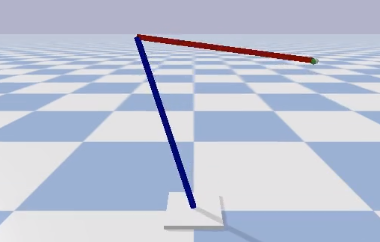
\includegraphics[width=.5\textwidth]{images/2DOF-robot.png}}}
  

\end{frame}
%===============================================================================


